\graphicspath{{Chapter6/Chapter6Figs/}}

\chapter{A modelling-experimental approach reveals IRS dependent regulation of AMPK by insulin}
\label{chap:A modelling-experimental approach reveals IRS dependent regulation of AMPK by insulin}
This chapter describes a systems biology-based investigation of AMPK regulation as described in \citep{Sonntag2012}. The results here focus on the modelling point of view and only include \emph{in vitro} experimental work necessary for model validation and test. All the \emph{in vitro} experimental data included in this project were collected by Annika Sonntag, PhD student supervised by Dr Kathrin Thedieck, Department of Bioinformatics and Molecular Genetics, Freiburg University, Germany. A copy of the published work, which includes the \emph{in vitro} experimental data used for parameterising and testing the model, is attached in Appendix \ref{appendixB}.

\section{Introduction}
\label{paper2-sec:Introduction}
After generating an insulin-mTOR dynamical model and determining mTORC2 induction by a distinct PI3K which is insensitive to the NFL \citep{DallePezze2012a}, the upstream regulation of both mTOR Complex 1 and 2 was elucidated and implemented. The next step was to add the energy signalling pathway, as represented by the AMPK module, into the model. \\
The choice of AMPK reflected the fact that this trimeric complex not only represents one of the most well known energy-dependent regulators within the cell \citep{Thedieck2009}, but also promotes, whereas mTORC1 inhibits, autophagy through ULK1 phosphorylation \citep{Lee2010, Kim2011} (see Section \ref{subsec:Roles of mTORC1 and AMPK in autophagy}). Under low energy conditions, AMPK directly phosphorylates and increases TSC2 GAPase activity \citep{Inoki2003}, thereby inhibiting mTORC1. In addition, AMPK phosphorylates the mTORC1 scaffold protein Raptor on two serine residues \citep{Gwinn2008}. This phosphorylation induces 14-3-3 binding to Raptor and is required for mTORC1 inhibition by energy deprivation. Therefore, the inclusion of AMPK into the model is essential for achieving a computational framework for both studying molecular mechanisms and achieving simulated drug interventions with the ultimate aim of extending lifespan. Further details concerning the biology of the energy signalling pathway can be 
found in Section \ref{subsec:The energy signalling pathway}. \\
In the process of data collection, we found that AMPK not only responds to energy deprivation but is also strongly activated by insulin within 3 minutes post induction, and is further induced in Raptor deficient cells. Although it was already shown that AMPK can be regulated by insulin \citep{Suzuki2004, Polak2008, Aguilar2007}, the mechanism involved in this regulation has not yet been clarified. The immunoblot-based AMPK-mTOR dynamical model was employed for generating a quality-of-fit based ranking of hypotheses of AMPK activation. This prediction using this procedure indicated that the most probable point in the network at which the insulin and AMPK signalling forked was at the level of IRS and that AMPK was dependent on the negative feedback loop (NFL). This was experimentally tested and confirmed in LKB1-deficient and -functional cells lines. In summary, this study shows that AMPK is positively regulated initially by IRS and inhibited by the NFL.
% Additional ORIGINAL TEXT
%mTOR does not only respond to the insulin network but is also connected to many other signalling cascades including AMP-dependent kinase (AMPK), Wnt-signalling, and the MEK/Erk pathway. To incorporate further kinase inputs into our dynamical network model we decided to focus on the development of an AMPK module. AMPK is activated by both energy deprivation and the kinase LKB1 (or STK11). Other kinases can phosphorylate AMPK-T172 independently of the cellular energy status, including Ca2+-sensitive calmodulin-dependent protein kinase kinase (CaMKK) [16-19] and TGFβ-activated kinase-1 (TAK1/MAP3K7) [20-22]. Also ataxia-telangiectasia mutated (ATM) kinase [23, 24] or inositol-requiring enzyme 1 (IRE1) [25] dependent induction of AMPK have been reported. 

\section{Results}
\label{paper2-sec:Results}
\subsection{An insulin-TOR-AMPK model}
\label{paper2-subsec:An insulin-TOR-AMPK model}
AMPK is another important mTOR regulator that suppresses mTORC1 activity in response to energy deprivation \citep{Mihaylova2011}. A new dynamical mTOR-AMPK model was generated including AMPK signalling to the earlier mTOR model as developed in \citep{DallePezze2012a} which only assumed insulin and amino acids as mTORC1 regulators. This new model implemented AMPK inhibition of mTORC1 through promotion of TSC1/TSC2 complex activity only. We chose not to include direct phosphorylation of Raptor by AMPK for two reasons: first, the AMPK functional regulation on mTORC1 was still maintained, since these two pathways both contributed to mTORC1 inhibition; second, the inclusion of a regulatory mechanism of Raptor and 14-3-3 was out of the scope of this project. The following new connection was added into the model presented in \citep{DallePezze2012a}: AMPK phosphorylation at T172 allows active AMPK to phosphorylate TSC2 at S1387 (species TSC1/TSC2) which leads to TSC1/TSC2 activity enhancement and subsequent inhibition of mTORC1 \citep{Inoki2003, Inoki2005, Mihaylova2011}. Conversely, the phosphorylation of TSC2 at T1462 (species TSC1/TSC2) by Akt-pT308 inhibits the TSC1/TSC2 complex, activating mTORC1 \citep{Inoki2002}. Finally, the species Akt-pS473, PRAS40-pT246 and PRAS40-pS183 were defined as supplementary readouts for mTORC2, Akt, and mTORC1, respectively. \\
Although AMPK is known to be induced by energy depletion \citep{Mihaylova2011}, AMPK was described to be induced in Raptor deficient cells \citep{Polak2008, Aguilar2007} and also gradually induced in gradual Raptor knock down HeLa cell line upon amino acids/insulin after only 20 min post induction (p.i.) (see \citep[Fig. 1A]{Sonntag2012}). Surprisingly, we found that insulin alone was able to strongly induce AMPK-pT172 and its readout TSC2-pS1387 already at 3 min p.i. and that these phosphorylations decreased over time. Although it has been described previously that AMPK is induced by IGF-1 \citep{Suzuki2004}, this signalling connection has to date only been poorly explored. Therefore, in the present study, the possible AMPK-activators in the insulin-mTORC1 signalling were systematically investigated. 
The AMPK activator candidates were selected among the upstream species of mTORC1 because: (1) mTORC1 is maximally induced at 30 - 45 min p.i. \citep{DallePezze2012a}, (2) AMPK induction by insulin peaked already as early as 3 min p.i., and (3) AMPK was induced by Raptor knockdown (e.g. mTORC1 inhibition). Therefore, we focused on the following AMPK activator candidates:
\begin{description}
 \item [Hypothesis 1 (Insulin)] where insulin is considered as a constant and direct input to AMPK;
 \item [Hypothesis 2 (IR\_beta\_pY1146)] reflecting IR activation;
 \item [Hypothesis 3 (IRS1\_p)] reflecting IRS1 activation by insulin receptor;
 \item [Hypothesis 4 (mTORC2\_pS2481)] reflecting mTORC2 activation by amino acids/insulin;
 \item [Hypothesis 5 (Akt\_pT308)] reflecting Akt activation downstream of PI3K;
 \item [Hypothesis 6 (TSC1\_TSC2\_pT1462)] reflecting TSC1/TSC2 deactivation by Akt.
\end{description}
A graphical representation of this insulin-mTOR-AMPK model depicting our six alternative hypotheses of AMPK activation is provided in Figure \ref{fig:fj_sb_12_0009_fig_1}. In order to add and calibrate the AMPK module, time course data for AMPK-pT172 and TSC1/TSC2-pS1387, monitoring the activity of AMPK and its readout TSC2, were acquired under serum and amino acids starvation followed by induction by insulin and amino acids, the same conditions used for calibration of the dynamic mTOR network model \citep{DallePezze2012a}. All signal intensities were quantified, and descriptive statistics were computed over three replicates. The experimental mean time courses were used to calibrate the model parameters.

\subsection{Parameter estimation and identifiability}
\label{paper2-subsec:Parameter estimation and identifiability}
A specific model was instantiated for each hypothesis and calibrated using the same data sets and using the Matlab Toolbox PottersWheel \citep{Maiwald2008}. Before calibrating the models, structural identifiability analysis was performed using the software GenSSI \citep{Chis2011}. This software calculated the symbolic solution of the problem computing Lie derivatives for each hypothesis confirming structural global identifiability for all six models.  For the IRS1-induced AMPK model, structural identifiability analysis is reported in Figure \ref{fig:fj_sb_12_0009_fig_2}A, showing that all the parameters were structurally identified in the first (blue circles) or second (magenta circles) order identifiability tableau.\\
To calibrate the models, experimental time course data upon amino acids/insulin induction for nine readouts (IR-beta-pY1146, IRS1-pS636, Akt-pT308, Akt-pS473, mTORC1-pS2448, mTORC2-pS2481, p70S6K-pT389, PRAS40-pT246, PRAS40-pS183; data set 1) in wild type cells along the insulin-mTOR signalling axis were used in combination with time course data under gradual mTORC1 inhibition (Raptor knock down; data set 2) in wild type cells, as measured previously \citep{DallePezze2012a}. Furthermore, in order to calibrate the species AMPK-pT172 and TSC1/TSC2-pS1387, the five  time points (0, 3, 20, 45, and 100 min. p.i.; \citep[Fig. 1A]{Sonntag2012}) without knock down induction, i.e. corresponding to wild type, were added as an additional data set (data set 3). \\
Parameter estimation was executed for each model independently over multiple data sets in order to reduce the bias of the solution and therefore overfitting. However, the addition of data sets used to calibrate a model can lead to a serious increment of variance, particularly due to the increase in intrinsic noise in experimental data, which does not permit to estimate the model correctly. Our second data set was characterised by three different levels of Raptor knock down, obtained by doxycycline treatment for 1, 2 or 3 days respectively (subsets 1-3). A satisfactory bias-variance trade off was found by combinatorially and singularly testing these three subsets and eventually selecting only the subset of Raptor knock down induced by doxycycline treatment for 3 days (subset 3). Subset 3 was selected as it represented the strongest signal reduction and consequently novel information with respect to wild type time courses (data set 1) for calibrating the model. Moreover, the readouts in our data sets (data set 
1, data set 2-subset 3, data set 3) were scaled in order to have species time course profiles of comparable intensity. This evenly distributes the cost of the solution over the simulated time course profiles approximating the data, avoiding an implicit preference ranking of calibration. \\
For calibrating the models, only the kinetic rate constant parameters were estimated, whereas the species protein concentrations were determined from immunoblot time course data sets by selecting the corresponding readout maximum intensity plus two standard deviations measured at that time point. The addition of two standard deviations to the maximum signal peak guaranteed to avoid species protein saturation conditions. The kinetic rate constants regulating PI3K-variant dynamics were fixed a priori assuming a time course similar to the insulin receptor. In fact, no experimental data is available for this PI3K insensitive to the negative feedback loop and it is more likely that it follows the IR-beta receptor than other curves. Furthermore, fixing these parameters led us to a full structural identifiability of the model.\\
A posterior identifiability analysis was performed using Mean Optimal Transformation Approach (MOTA) plugin \citep{Maiwald2008, Hengl2007} after selecting 50\% of the best fits (shown in Figure \ref{fig:fj_sb_12_0009_fig_2}B for the IRS1-induced AMPK model). This analysis revealed that high parameter correlations had coefficient of variation (CV) lower than 0.05 for all our models except for the IR -beta-induced AMPK model (Hypothesis 2; Figure \ref{fig:fj_sb_12_0009_supp_fig_1}). For this model, MOTA analysis highlighted high correlation and CV for the pair of parameters regulating AMPK dynamics. Model identifiability was obtained after fixing one of the two parameters and recalibrating the remaining one in a second round of calibration. In combination with the previous analysis, parameter non-identifiability was also checked by directly analysing the estimated percentage of standard deviations of the parameters, computed over the 50\% best fits, and considering non-identifiable the parameters with 
standard deviations higher than a threshold of 5\%. Table \ref{tab:fj_sb_12_0009_fig_t1} presents the estimated parameters values with mean, standard deviations and CV for the IRS1-induced AMPK model showing parameter identifiability. Sensitivity analysis for the same model is provided in Figure \ref{fig:fj_sb_12_0009_supp_fig_2}, showing a balanced sensitivity among the parameters and that all of them were required.\\
In summary, six models sharing the main network structure and differing in AMPK activation were independently calibrated. The next step was therefore to find at which level in the network AMPK is induced by insulin. 

\subsection{Hypotheses ranking and testing of AMPK activation by insulin}
\label{paper2-subsec:Hypotheses ranking and testing of AMPK activation by insulin}
Once parameter estimation was achieved, the simulated time courses for the readouts AMPK-pT172 and TSC1/TSC2-pS1387 of each model were compared with the corresponding experimental time courses (see Figure \ref{fig:fj_sb_12_0009_fig_3}). Surprisingly, the readouts AMPK-pT172 and TSC1/TSC2-pS1387 for the IRS1-induced AMPK model (Hypothesis 3) were found to fit the data with high accuracy, whereas the goodness-of-fit decreased for species downstream of IRS1 (Akt and TSC1/TSC2; Hypotheses 5 and 6) and upstream of IRS1 (Insulin, IR-beta; Hypotheses 1 and 2), as indicated by the measure $\chi^2$. Furthermore, the two readouts fitted worse for the mTORC2-induced AMPK model (Hypothesis 4). \\
At this point, the question was whether these local differences could lead to a possible ranking of the overall models. In order to achieve this, several additional likelihood-based statistical criteria, such as Akaike Information Criterion (AIC, AICc) \citep{Akaike1973} and Bayesian Information Criterion (BIC) \citep{Schwarz1978}, were used besides the total $\chi^2$, to estimate the goodness-of-fit calculated over the entire models. Through these estimations a ranking of the hypotheses in according to the goodness-of-fit was established (see Table \ref{tab:fj_sb_12_0009_fig_t2}). All these measures were consistent between them in selecting the IRS1-induced AMPK model (Hypothesis 3) as the most probable model. The remaining simulated versus experimental time courses for IRS1-induced AMPK model are reported in Figure \ref{fig:fj_sb_12_0009_supp_fig_3}. An SBML model is provided for the IRS1-induced AMPK hypothesis.\\
In order to test hypotheses ranking and specifically Hypothesis 3 validity, four experimental tests were conducted: IRS over-expression, PI3K inhibition by Wortmannin, PTEN over-expression and myristoylated Akt. Schematic diagrams illustrating these tests are provided in Figure \ref{fig:paper2_schematic_diagrams_tests}. These tests consistently confirmed the predicted validity of Hypothesis 3, rejecting all the other hypotheses and are in line with the observed AMPK induction in mTORC1 deficient cells (see \citep{Aguilar2007, Polak2008}). Moreover, since HeLa cells do not express AMPK upstream kinase LKB1 \citep{Suzuki2004,Sun2007}, this mechanism of AMPK induction by insulin was also tested and confirmed in C2C12 cell line, which is LKB1 functional. Experimental testing details can be found in \citep[Fig. 4]{Sonntag2012}. A graphical representation of the IRS1-induced AMPK model (Hypothesis 3) in SBGN notation is given in Figure \ref{fig:fj_sb_12_0009_fig_5}.

\section{Discussion}
\label{paper2-sec:Discussion}
In the present study, amino acids/insulin was observed to induce AMPK, confirming a previous report \citep{Suzuki2004}. Here, we showed that this induction happened already at 3 minutes post treatment with amino acids/insulin and increased under Raptor inhibition. The dynamical model developed in \citep{DallePezze2012a} was employed and extended with an AMPK module. This work systematically explored which component in the IIS-TOR signalling pathway was the most likely candidate activator of AMPK. Applying a hypothesis ranking based on quality-of-fit between the model and experimental data sets, a signalling fork was predicted at the level of IRS (Hypothesis 3), one fork leading to the canonical insulin signalling pathway, another one to AMPK. This prediction was experimentally confirmed in LKB1-deficient (HeLa) and -functional (C2C12) cells lines. Besides confirming this hypothesis, experimental tests also rejected all the other hypotheses, which were already considered less probable by our predictions due 
to poor fitting with the data. These results showed that AMPK induction was dependent on IRS and was therefore sensitive to the NFL, in agreement with our previous finding that Raptor inhibition increased AMPK activation.\\
From a modelling point of view, a comprehensive mTOR network has been studied statically \citep{Caron2010} and parts of the mTOR network have been modelled dynamically \citep{Sedaghat2002, Jain2009, Faratian2009, Vinod2009, Borisov2009, Kuepfer2007, Kiselyov2009, DallePezze2012a}. The network presented in this study is the most extensive mTOR-AMPK model, incorporating AMPK as directly regulated by amino acids/insulin. Six models were defined and calibrated using our experimental data. The models shared the main network structure, but differed for the AMPK activation mechanism. After repeating cycles of parameter calibration and identifiability for each model, likelihood-based statistical measures were used to estimate a model ranking, based on the goodness-of-fit between each model and the experimental data.\\
Interestingly, other studies reported that AMPK inhibits IRS by phosphorylation of IRS1 at S794 \citep{Ning2010, Tzatsos2007, Jakobsen2001}. What is the meaning of this inhibition along with the activation mechanism reported in this study? May this be an additional mechanism to switch off the insulin signalling analogous with the canonical IIS-TOR signalling and the p70-S6K-induced negative feedback loop? A possible explanation of this redundancy may be to increase the robustness of the cellular system upon insulin stimulation. Certainly, further investigation on the dual regulation of AMPK and IRS is required in order to better characterise the role of IRS and the meaning of its downstream effect on AMPK.\\
In this study, we found that AMPK activation was dependent on IRS in HeLa cells, which are known to be LKB1-deficient, and confirmed this results in C2C12 cells line, which are LKB1-functional cells. Another study reported that IGF1 could induce AMPK in LKB1-functional PANC1 cells, besides HeLa cells \citep{Suzuki2004}. Therefore, the activation of AMPK at the level of IRS, presented in this work, could be conserved in other cells in addition to HeLa, C2C12 and PANC1.\\
Finally, linking AMPK with IRS1 and the NFL is a crucial aspect in drug intervention, since the positive effects of AMPK activity can be maximised by mTOR-inhibitors \citep{GarciaEcheverria2011}. In this context, model simulations of drug treatments can offer a parsimonious and rapid methodology for predicting best protein-dependent drug intervention and administration in preventing or treating metabolic and tumour diseases.


\section{Materials and methods}
\label{paper2-sec:Materials and methods}
\subsection{Modelling}
\label{paper2-subsec:Modelling}
The illustrated graphical model in SBGN graphical notation \citep{lenovere2009systems} were designed using CellDesigner 4.2 \citep{Funahashi2003, Funahashi2008}. The Matlab Toolbox PottersWheel \citep{Maiwald2008} was used for designing and calibrating the models. The parameters for each of the models were estimated by 1000 fits with parameter disturbance noise of 0.4 using the best fit as starting value. For each fit a maximum of 250 iterations with $\chi^2$ and parameters tolerances of 1e-07 were run using the optimisation algorithm TrustRegion. To reduce the computation time, CVODES integrator was selected and configured with the following parameters: maximum number of steps = 1500, relative tolerance = 1e-06, absolute tolerance = 1e-08. 
The reactions representing the dynamics of the models were described by mass action laws. Only the kinetic rate constants were estimated and the interval [1e-06, 1e+04] was selected as a constraint for each parameter. The initial protein concentrations were directly determined from our experimental data and scaled to distribute the fitting quality over the model. Experimental error bars indicate standard error of the mean (SEM). The dynamics for the species PI3K-variant were assumed by reproducing the dynamics of the insulin receptor, whereas its initial concentration was the same as IRS1 species. \\
Structural identifiability was calculated a priori with GenSSI \citep{Chis2011}. The model in Potterswheel format was exported in SBML and converted to Octave format using The System Biology Format Converter (SBFC)\footnote{Software available from \href{http://sourceforge.net/}{http://sourceforge.net/}}. Then the model in Octave format was adapted for the software GenSSI. Symbolic solutions for each model were computed setting 10 as maximum number of iterations. After executing each sequence fits, parameters were considered non-identifiable when their coefficients of variance (CV), measured in the best 50\% fits of the calibration sequence, were higher than 5\%. In combination to this preliminary analysis, the PottersWheel plugin MOTA was used to confirm the parameter non-identifiability and to assess the relations between the target parameter and the others. \\
3D Sensitivity analysis was performed using PottersWheel and provided in Figure \ref{fig:fj_sb_12_0009_supp_fig_2}. Models were exported in SBML \citep{hucka2003systems} Level 2 Version 4 using PottersWheel.

\subsection{Statistics}
\label{paper2-subsec:Statistics}
The Standard Error of the Mean (SEM) was chosen to estimate the statistical variability of the measured samples of experimental time course. The goodness-of-fit statistical measures $\chi^2$ \citep{Maiwald2008}, AIC, AICc \citep{Akaike1973} and BIC \citep{Schwarz1978} were used in order to rank the hypotheses. All these measures were directly computed using PottersWheel Toolbox. The statistical and programming language R v. 2.13.1 \citep{RCoreTeam} was selected for the graphic representation of the identifiability matrix computed with MOTA and for all the computed statistics.


\section{Figures and tables}
\label{paper2-sec:Figures and tables}

\begin{figure}[tb]
	\begin{center}
		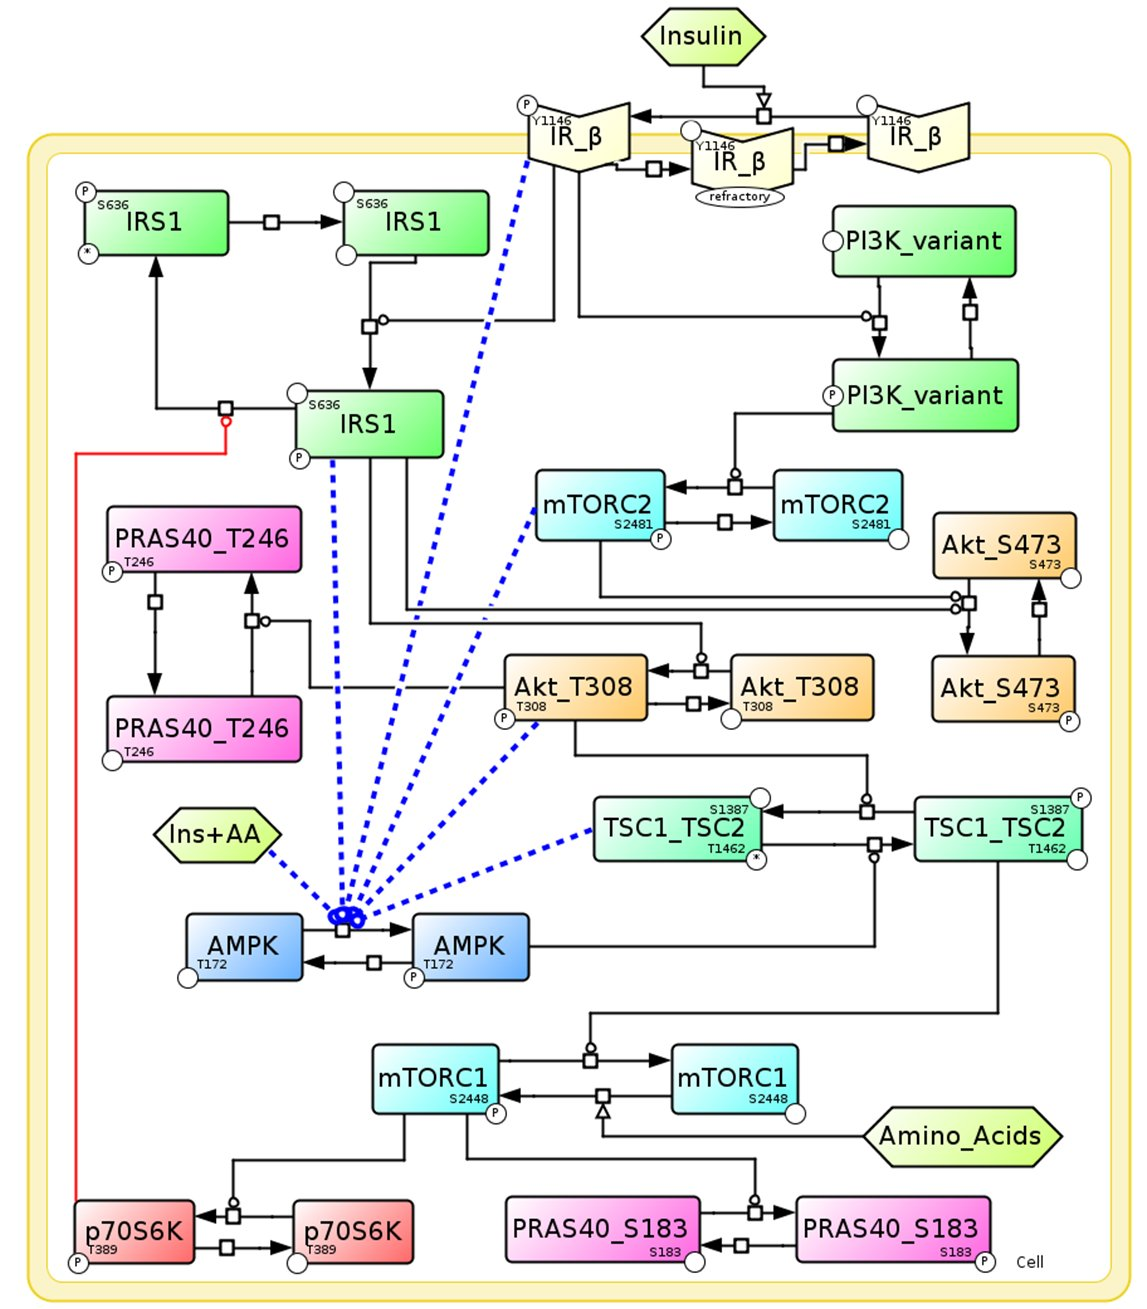
\includegraphics[scale=1.25]{fj_sb_12_0009_fig_1.jpg}
		\caption[Graphical insulin-mTOR-AMPK model]{Graphical insulin-mTOR-AMPK model. This model integrates the insulin-mTOR model presented in \citep{DallePezze2012a} with AMPK regulation. Six hypotheses of AMPK activation are investigated (blue dotted lines). Except for the Insulin- and IR-beta-induced AMPK hypotheses, all the others implicitly assume AMPK being dependent on the p70-S6K-negative feedback loop.}
		\label{fig:fj_sb_12_0009_fig_1}
	\end{center}
\end{figure}
\clearpage

\begin{figure}[tb]
	\begin{center}
		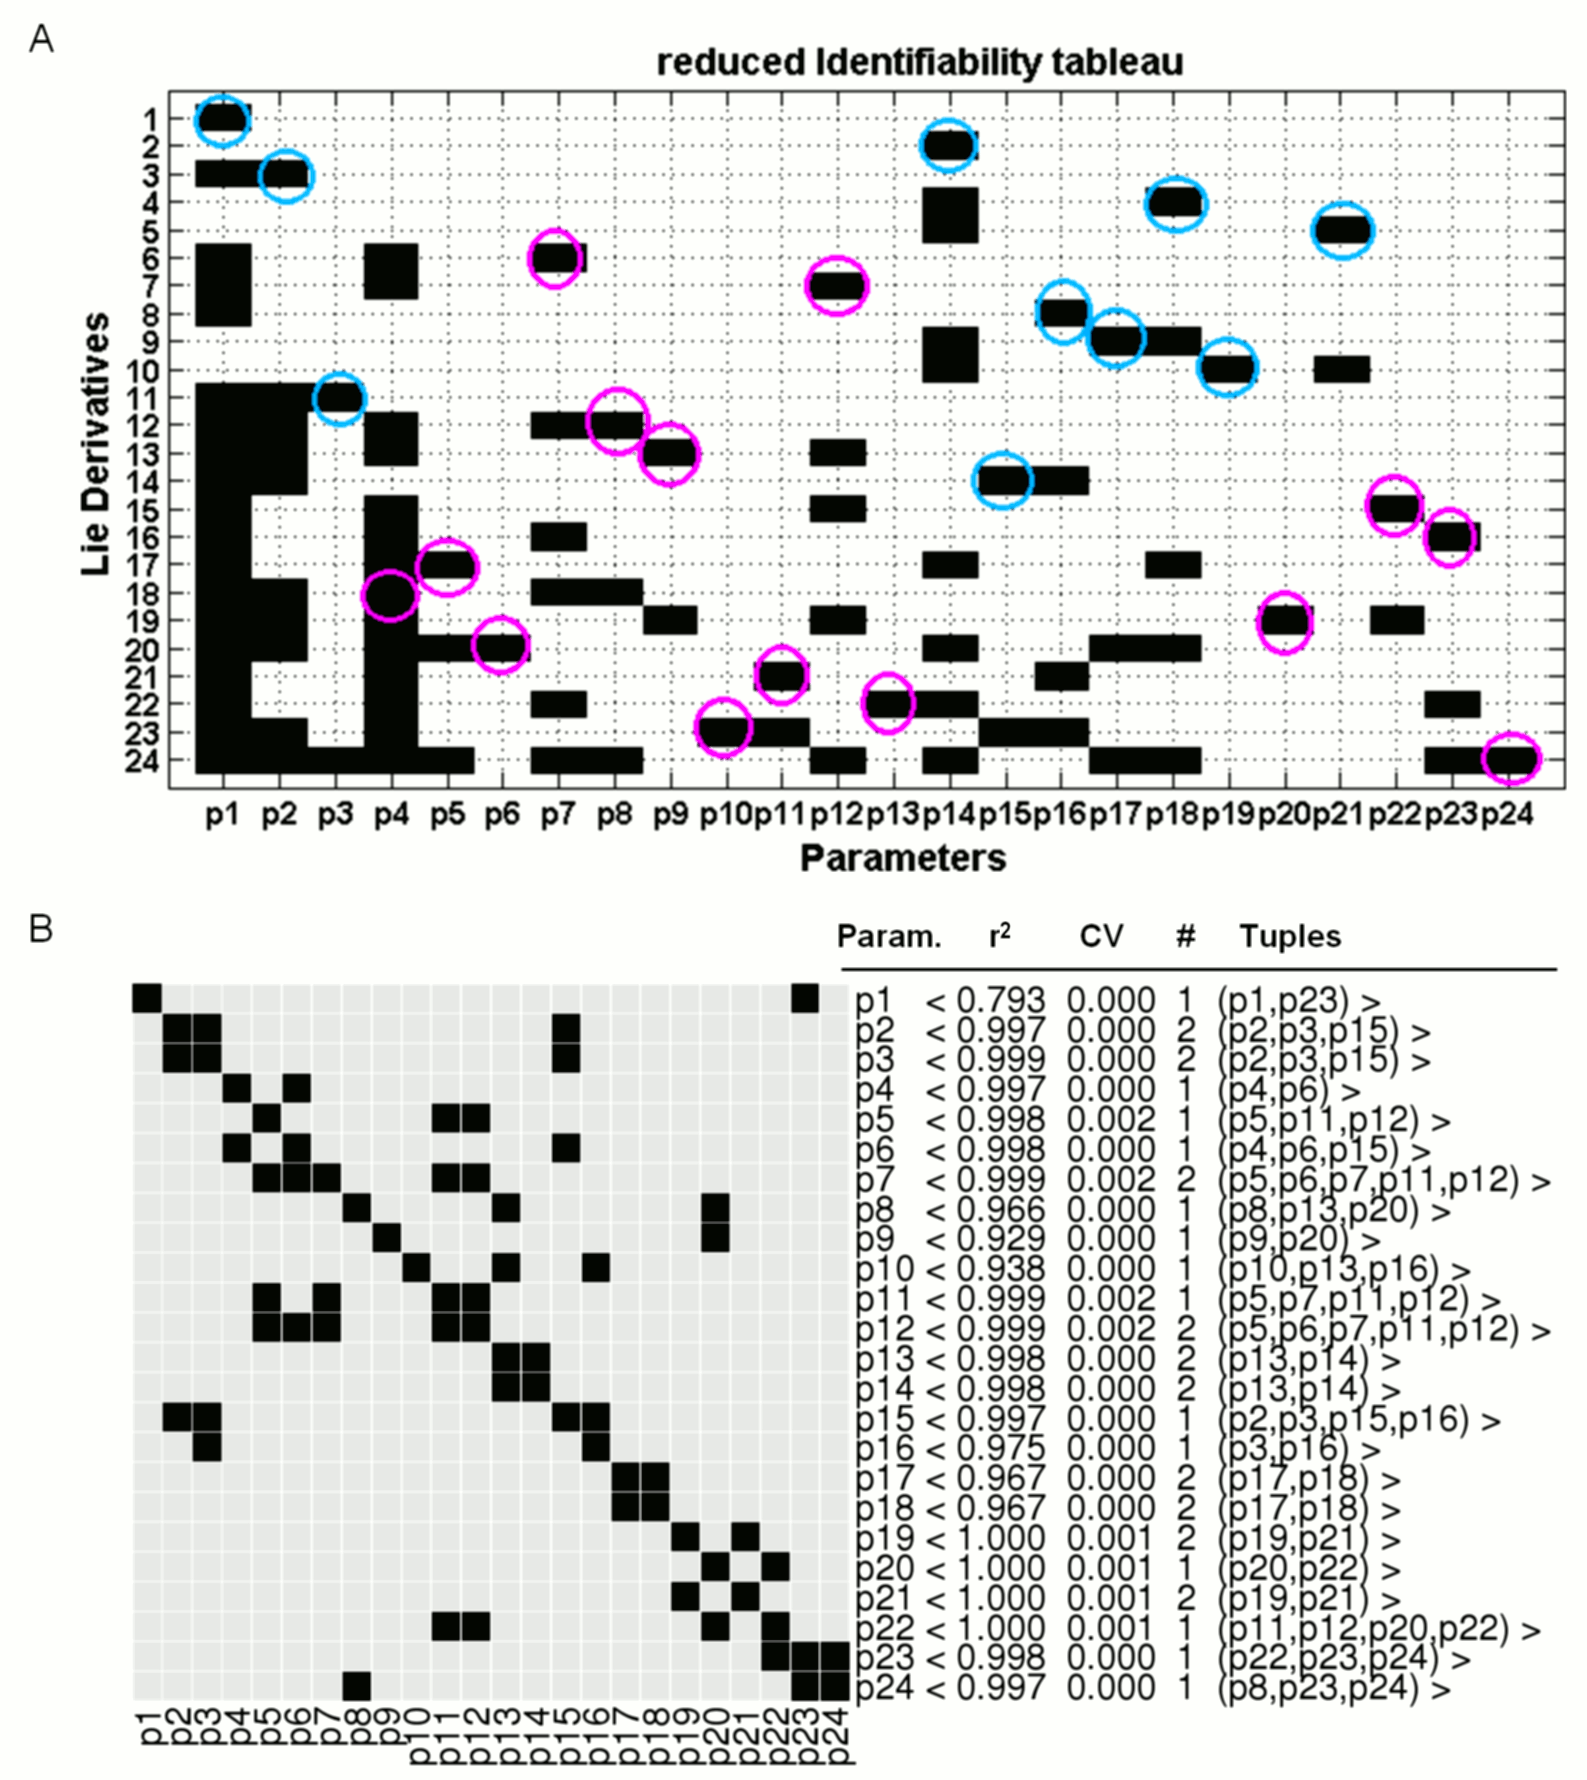
\includegraphics[scale=0.9]{fj_sb_12_0009_fig_2.png}
		\caption[Identifiability analysis for IRS1-induced AMPK model (Hypothesis 3)]{Identifiability analysis for IRS1-induced AMPK model (Hypothesis 3). (A) Structural identifiability analysis was performed with the software GenSSI a priori. In the reduced identifiability tableau, blue circles indicate the parameters detected directly as structurally globally identifiable at the first order tableau, whereas magenta circles highlight the parameters detected as structurally globally identifiable at the second order tableau after computing the symbolic solution. (B) MOTA identifiability analysis was executed using the 50\% of the best fits of the calibration fits sequence. A correlation among a set of parameters is indicated by the tuple of correlated parameters, their correlation coefficient ($r^2$), coefficient of variation ($CV$) and the number of times this correlation is identified by varying the parameters of the tuple ($\#$). Even though there are high correlations among some parameters, the corresponding 
coefficient of variation was lower than 0.002, which can be explained as numeric approximation error in the fit sequence calibration process. (*) $r^2 > 0.9$ \& $CV > 0.1$  (**) $r^2 > 0.9$ \& $CV > 0.1$ \& \#$> 1$.}
		\label{fig:fj_sb_12_0009_fig_2}
	\end{center}
\end{figure}
\clearpage

\begin{figure}[tb]
	\begin{center}
		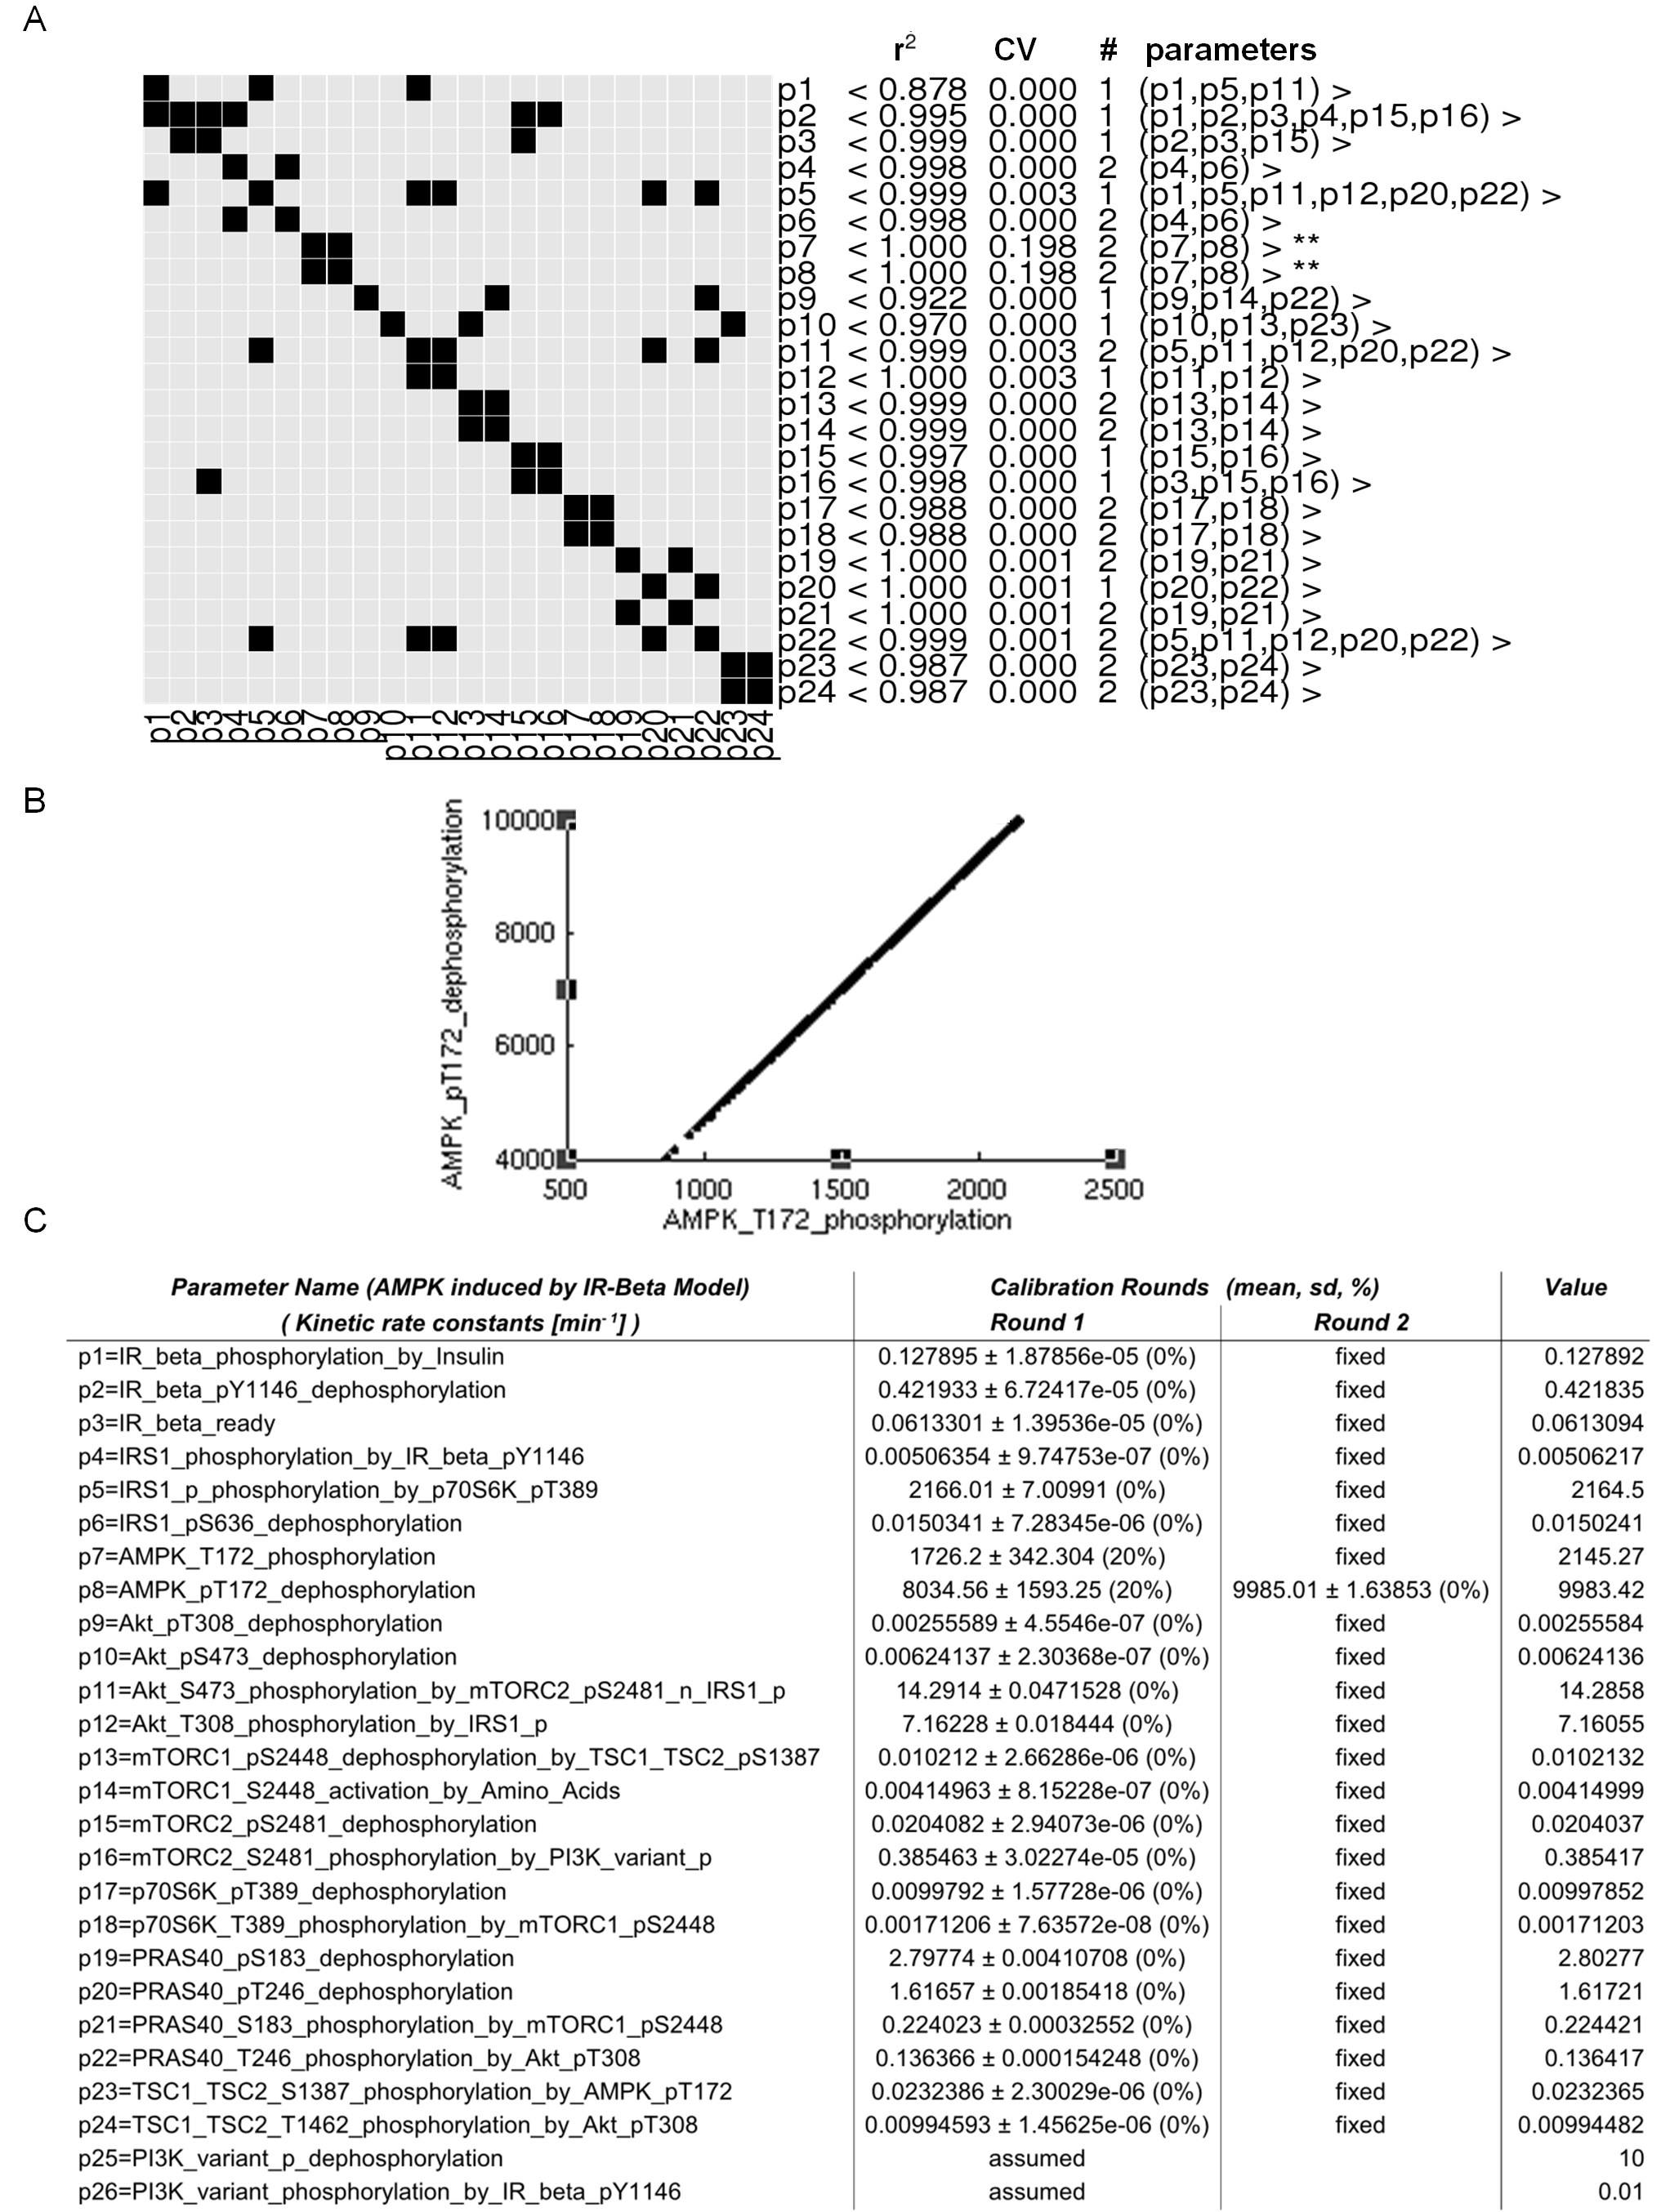
\includegraphics[scale=0.70]{fj_sb_12_0009_supp_fig_1.png}
		\caption[Identifiability and parameter estimation for IR-beta-induced AMPK model (Hypothesis 2)]{Identifiability and parameter estimation for IR-beta-induced AMPK model (Hypothesis 2). (A) Identifiability analysis for the IR-beta-induced AMPK model indicated non identifiability issues for the parameters regulating AMPK dynamics (p7, p8). (B) Correlation plot between the two parameters (p7, p8) confirms non-identifiability of the parameters. (C) Finally, the first round of the parameter estimation reported a standard deviation percentage higher than 5\% for the two parameters. p8 was further recalibrated in a second round in which it was correctly identified. (*) $r^2 > 0.9$ \& $CV > 0.1$  (**) $r^2 > 0.9$ \& $CV > 0.1$ \& \#$> 1$.}
		\label{fig:fj_sb_12_0009_supp_fig_1}
	\end{center}
\end{figure}
\clearpage

\begin{figure}[tb]
	\begin{center}
		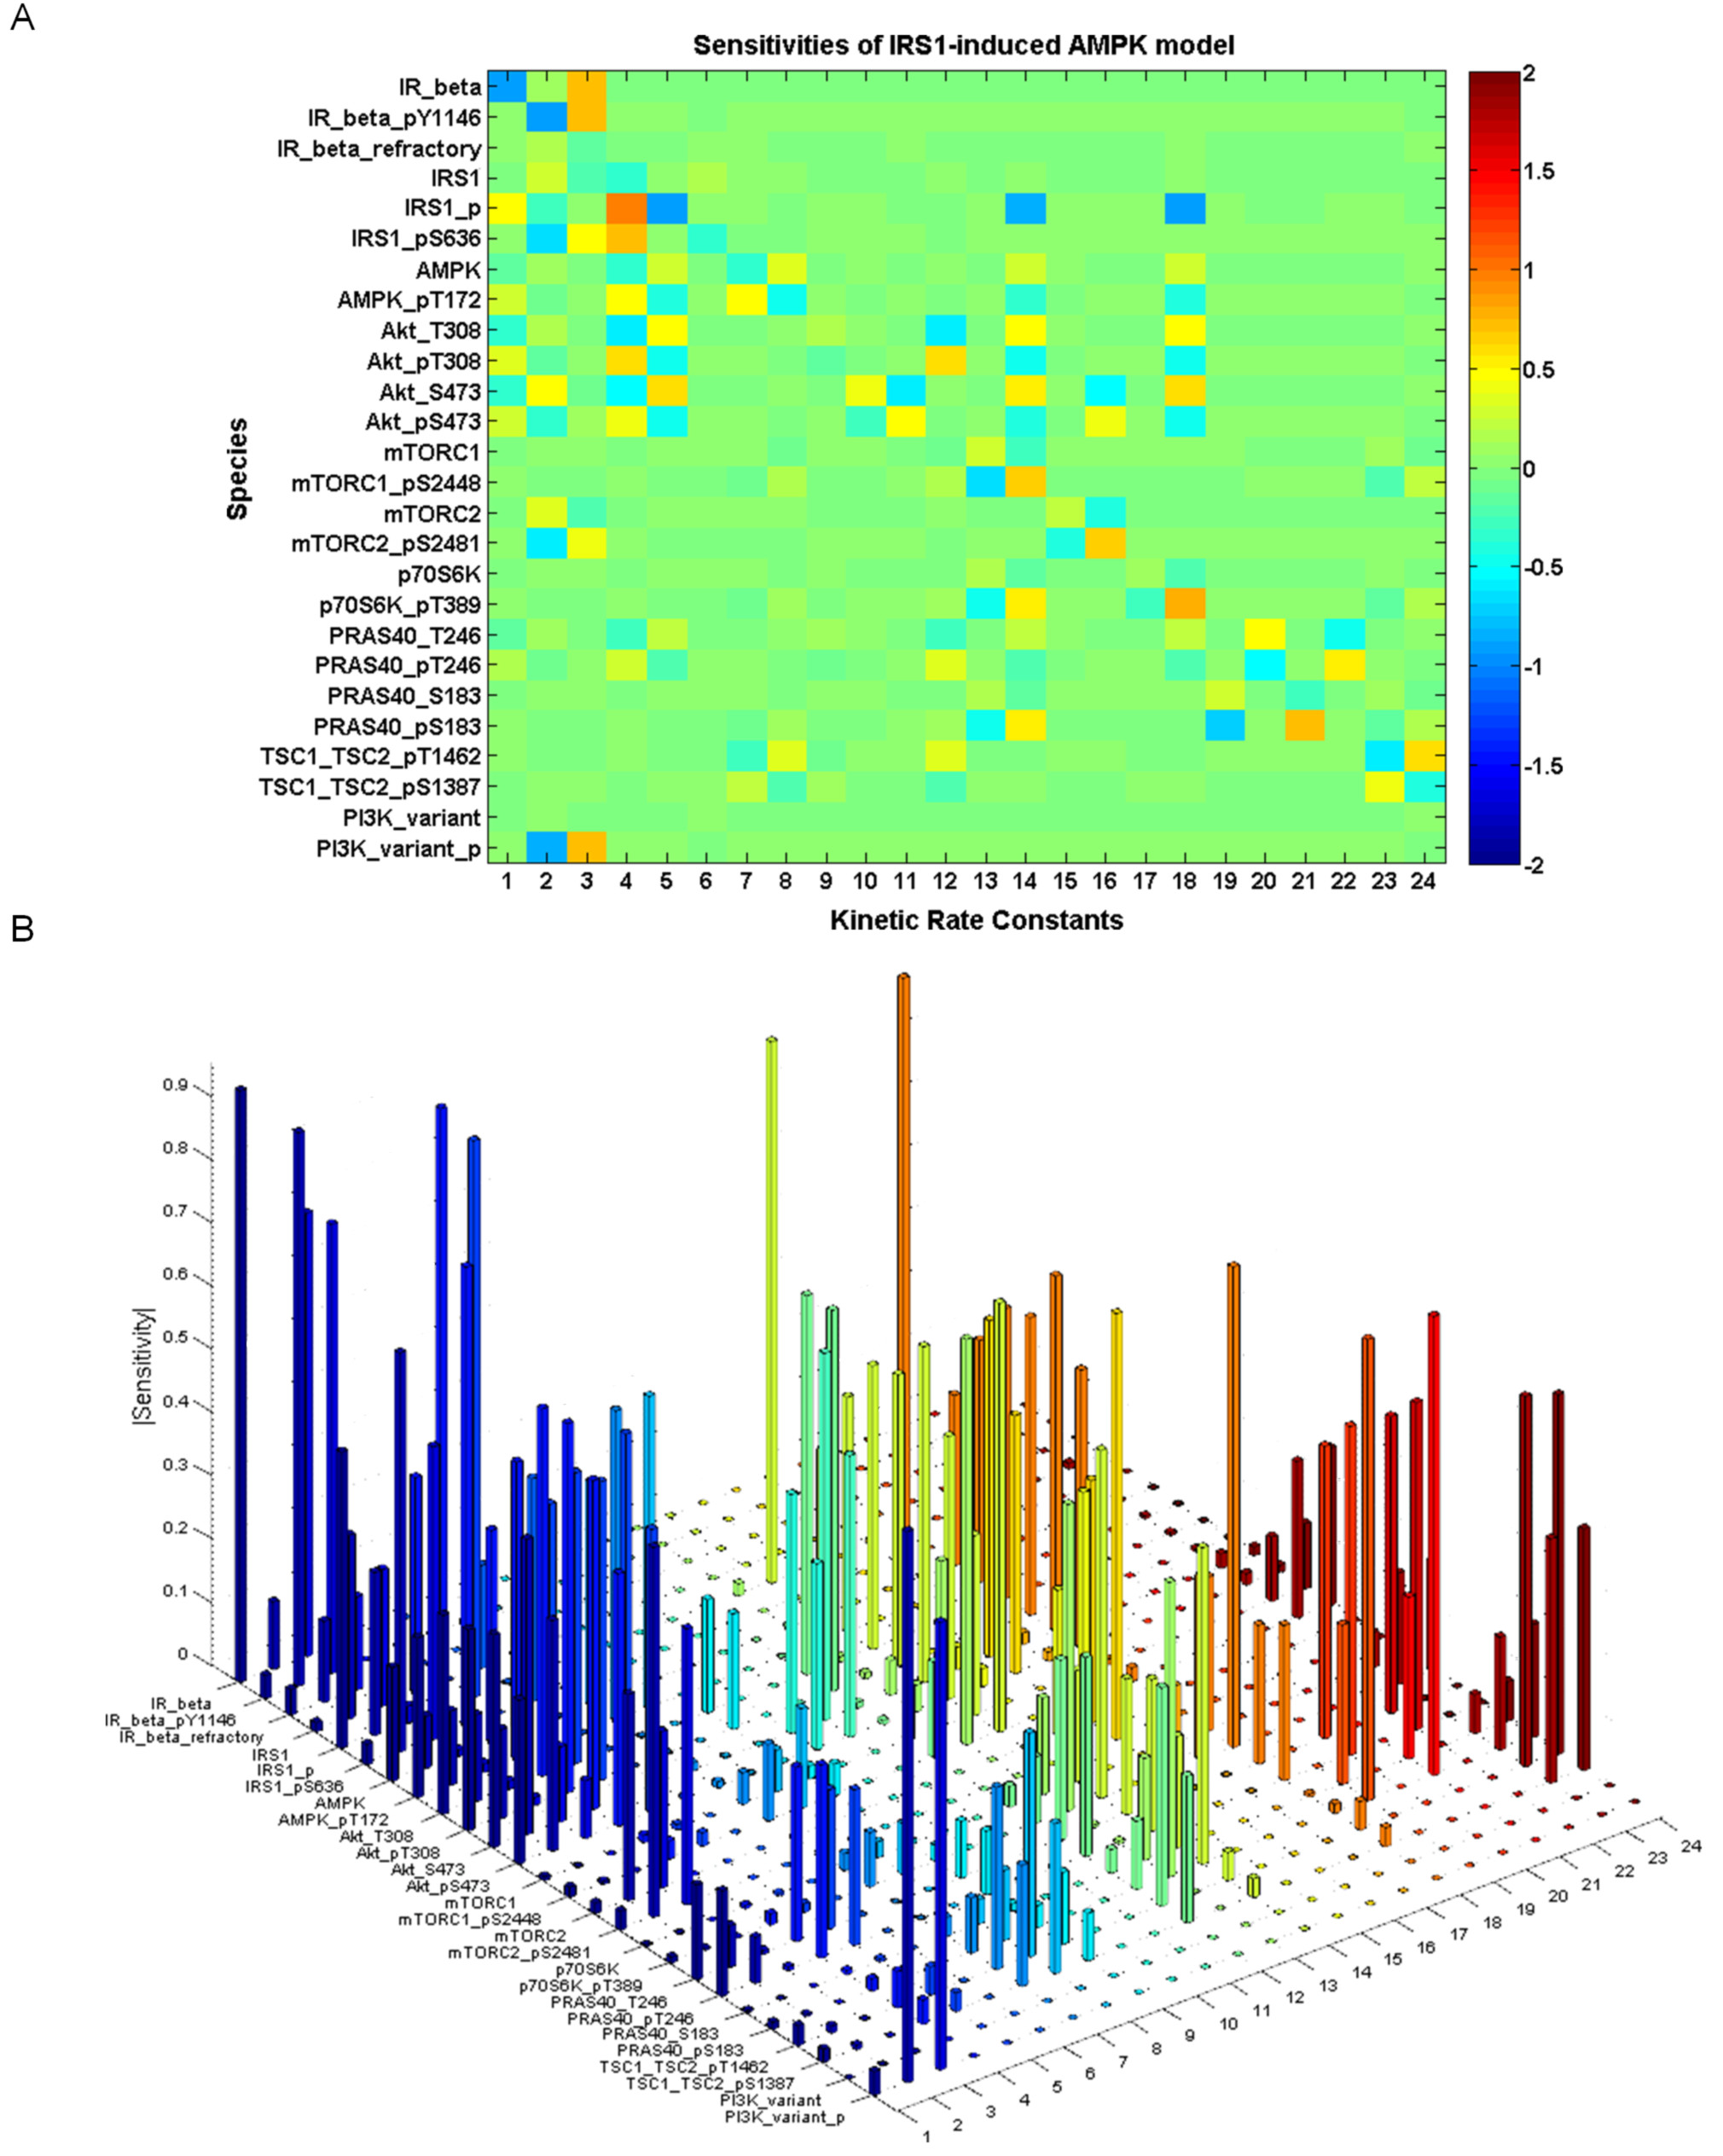
\includegraphics[width=5.35in]{fj_sb_12_0009_supp_fig_2.jpg}
		%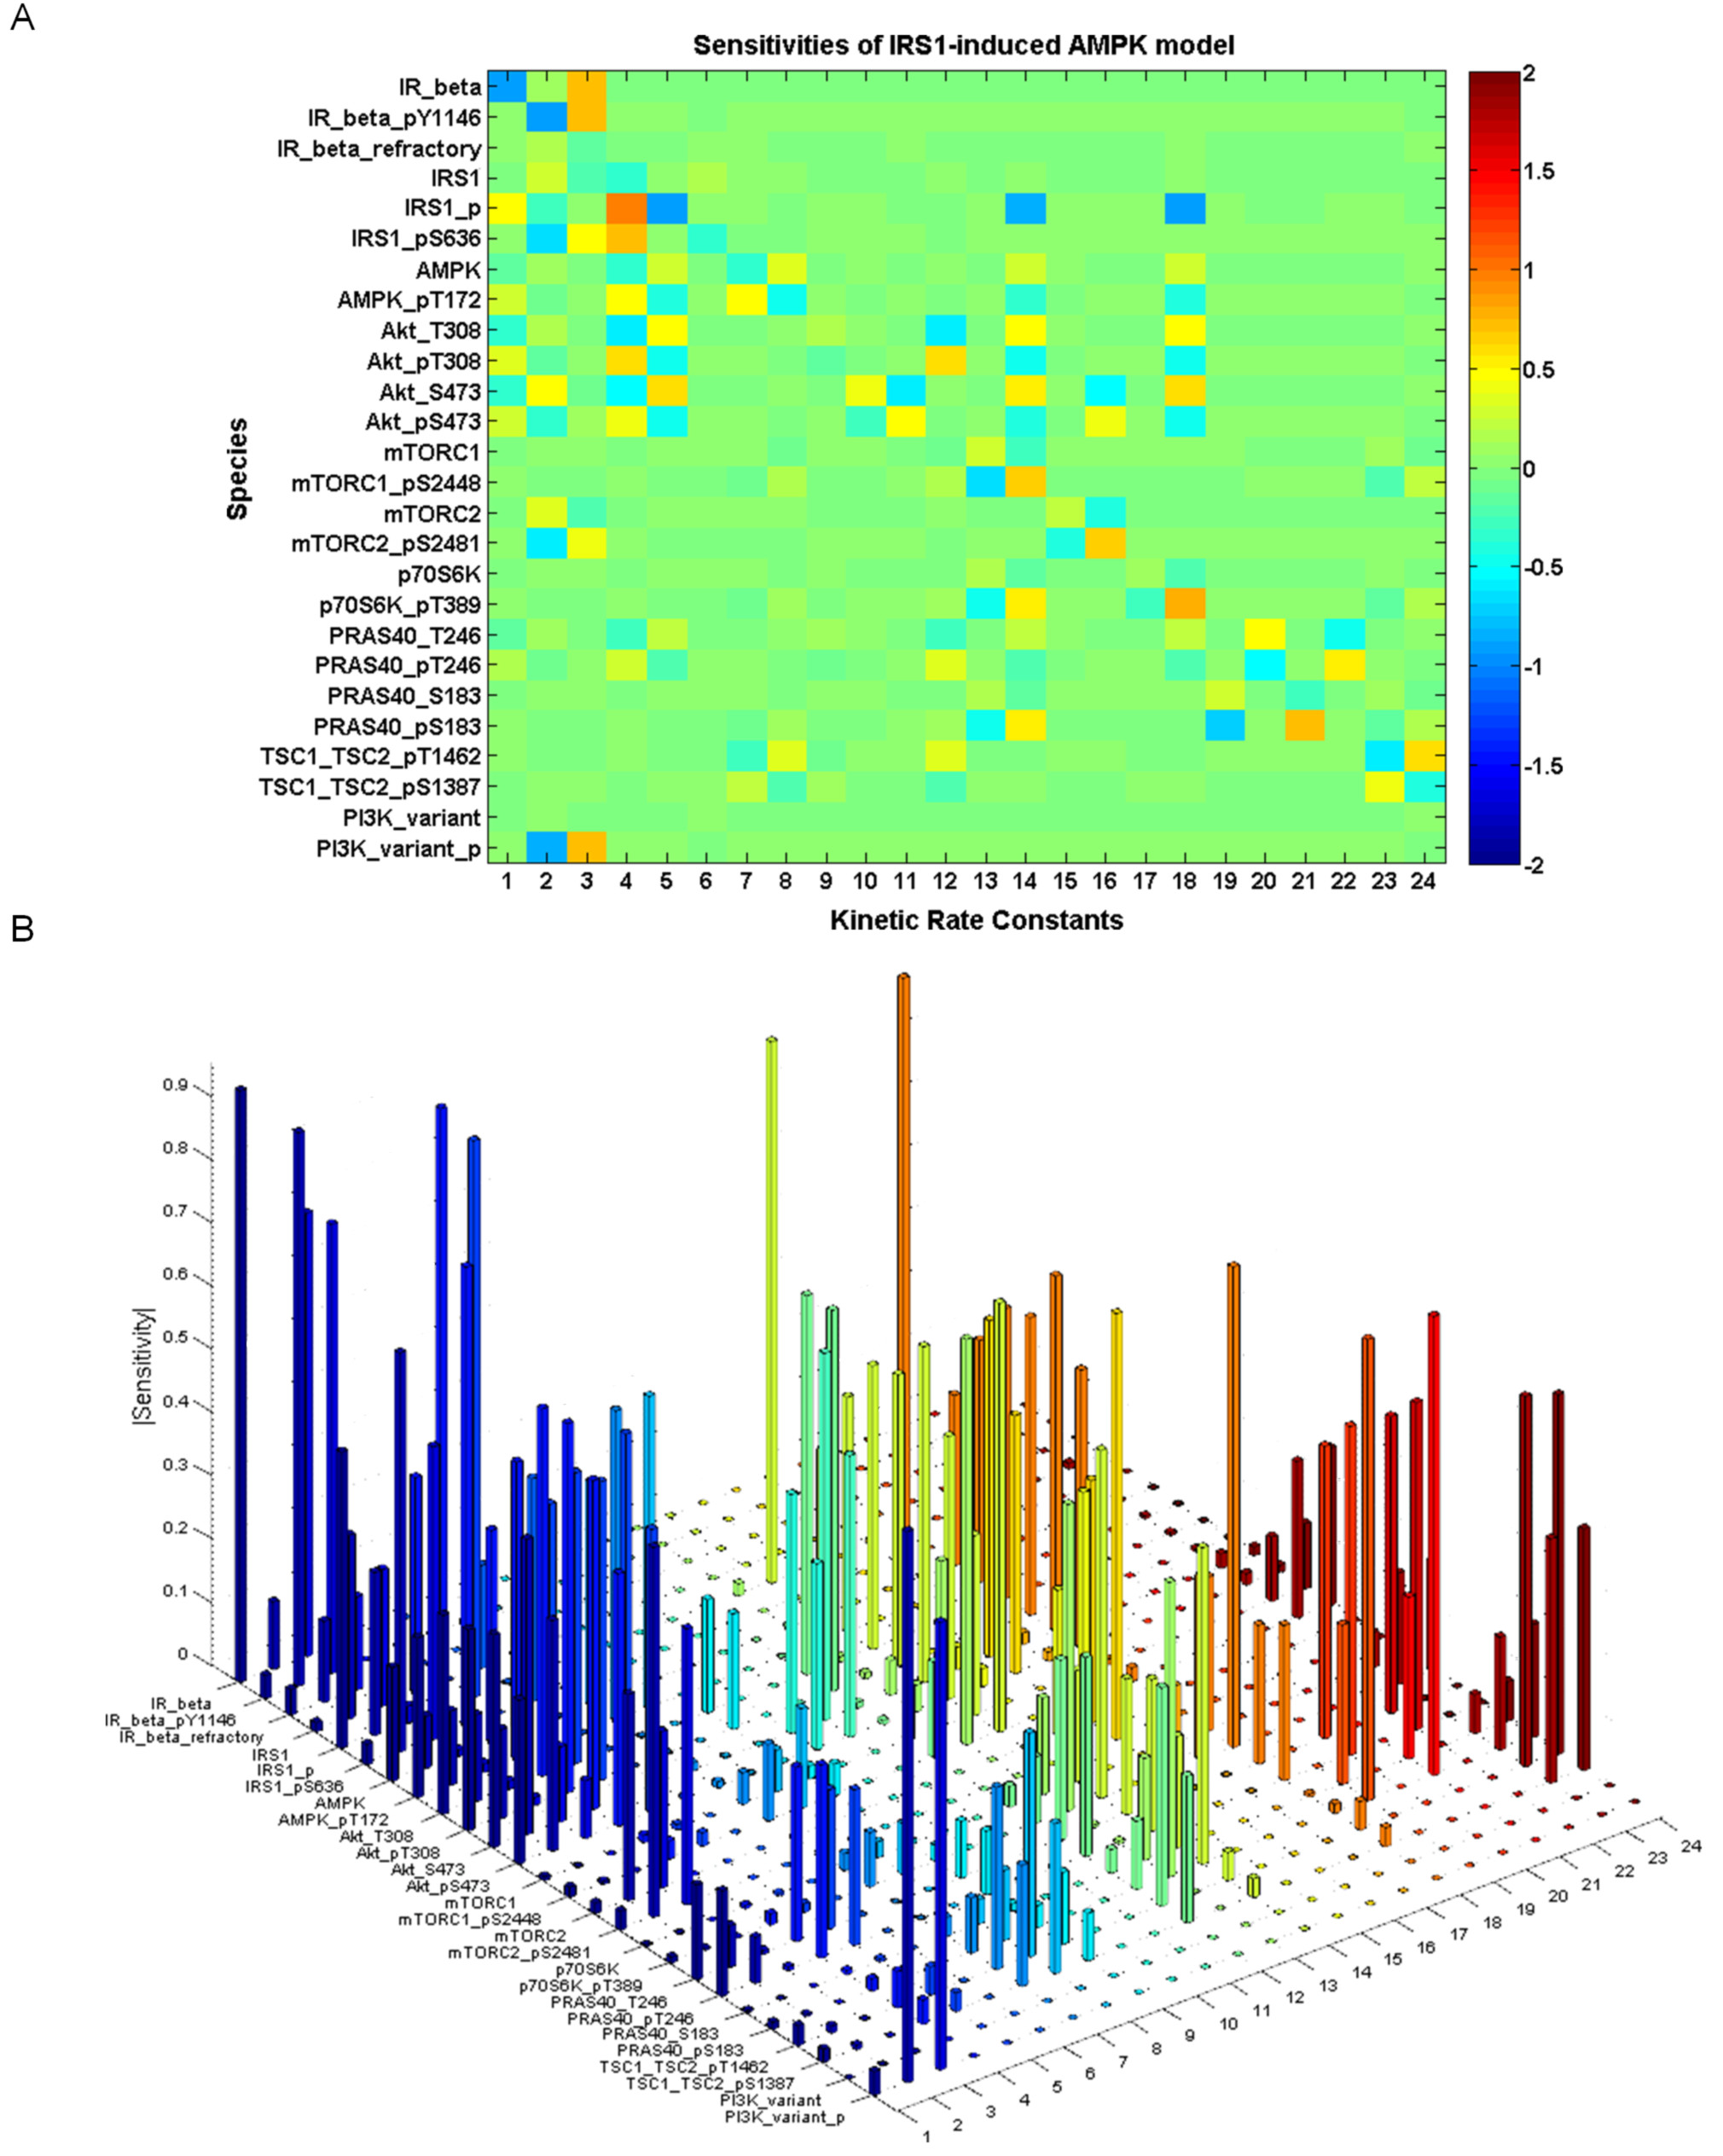
\includegraphics[scale=0.75]{fj_sb_12_0009_supp_fig_2.jpg}
		\caption[Sensitivity analysis for IRS1-induced AMPK model (Hypothesis 3)]{Sensitivity analysis for IRS1-induced AMPK model (Hypothesis 3). (A) 2-dimensional sensitivity analysis between the estimated kinetic rate constants versus the protein concentrations. The table shows that all the parameters are essential for describing the model and the IRS1-p regulation is the most important as it mediates the insulin signalling as well as the p70-S6K-negative feedback loop. Colours indicate sensitivity levels. (B) 3-dimensional sensitivity analysis as normalised in [0,1]. Colours distinguish different estimated kinetic rate constant parameters.}
		\label{fig:fj_sb_12_0009_supp_fig_2}
	\end{center}
\end{figure}
\clearpage

\begin{figure}[tb]
	\begin{center}
		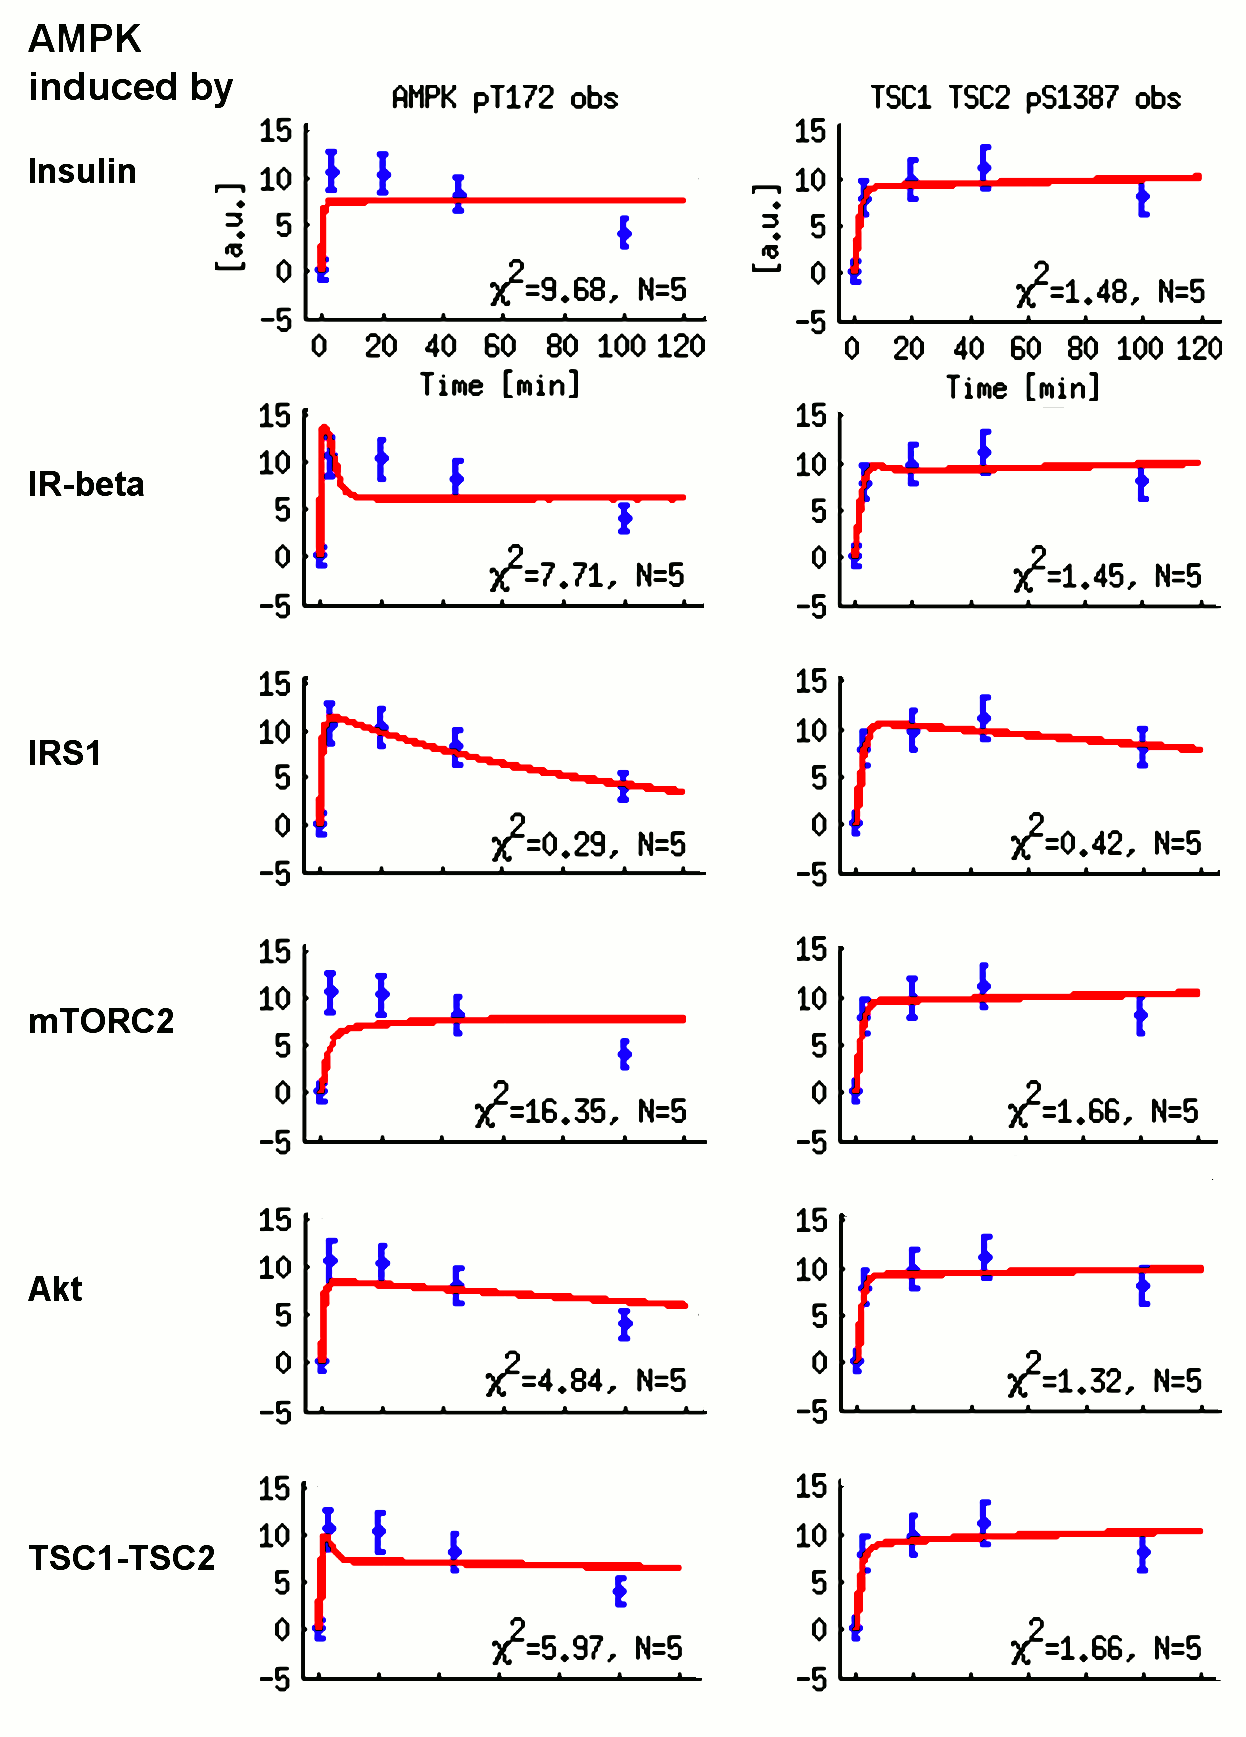
\includegraphics[scale=0.95]{fj_sb_12_0009_fig_3.png}
		\caption[Prediction of the intersection between insulin and AMPK signalling]{Prediction of the intersection between insulin and AMPK signalling. Simulated time courses (red lines) versus experimental data (blue points) for AMPK-pT172 and its downstream readout TSC1/TSC2-pS1387 (columns) shown for the six hypotheses: Insulin-, IR-beta-, IRS-, mTORC2-, Akt-, TSC1/TSC2-induced AMPK (rows). These predictions suggest that AMPK could be regulated by kinases downstream of the insulin receptor. The IRS-induced AMPK model (Hypothesis 3) fitted experimental data best. Experimental data error bars indicate standard error of the mean (SEM) calculated from three repetitions. Goodness-of-fit $\chi^2$ is reported for each plot along with the number of measured time points. \emph{In vitro} experiments were performed by Annika Sonntag, Freiburg University, Germany.}
		\label{fig:fj_sb_12_0009_fig_3}
	\end{center}
\end{figure}
\clearpage

\begin{figure}[tb]
	\begin{center}
		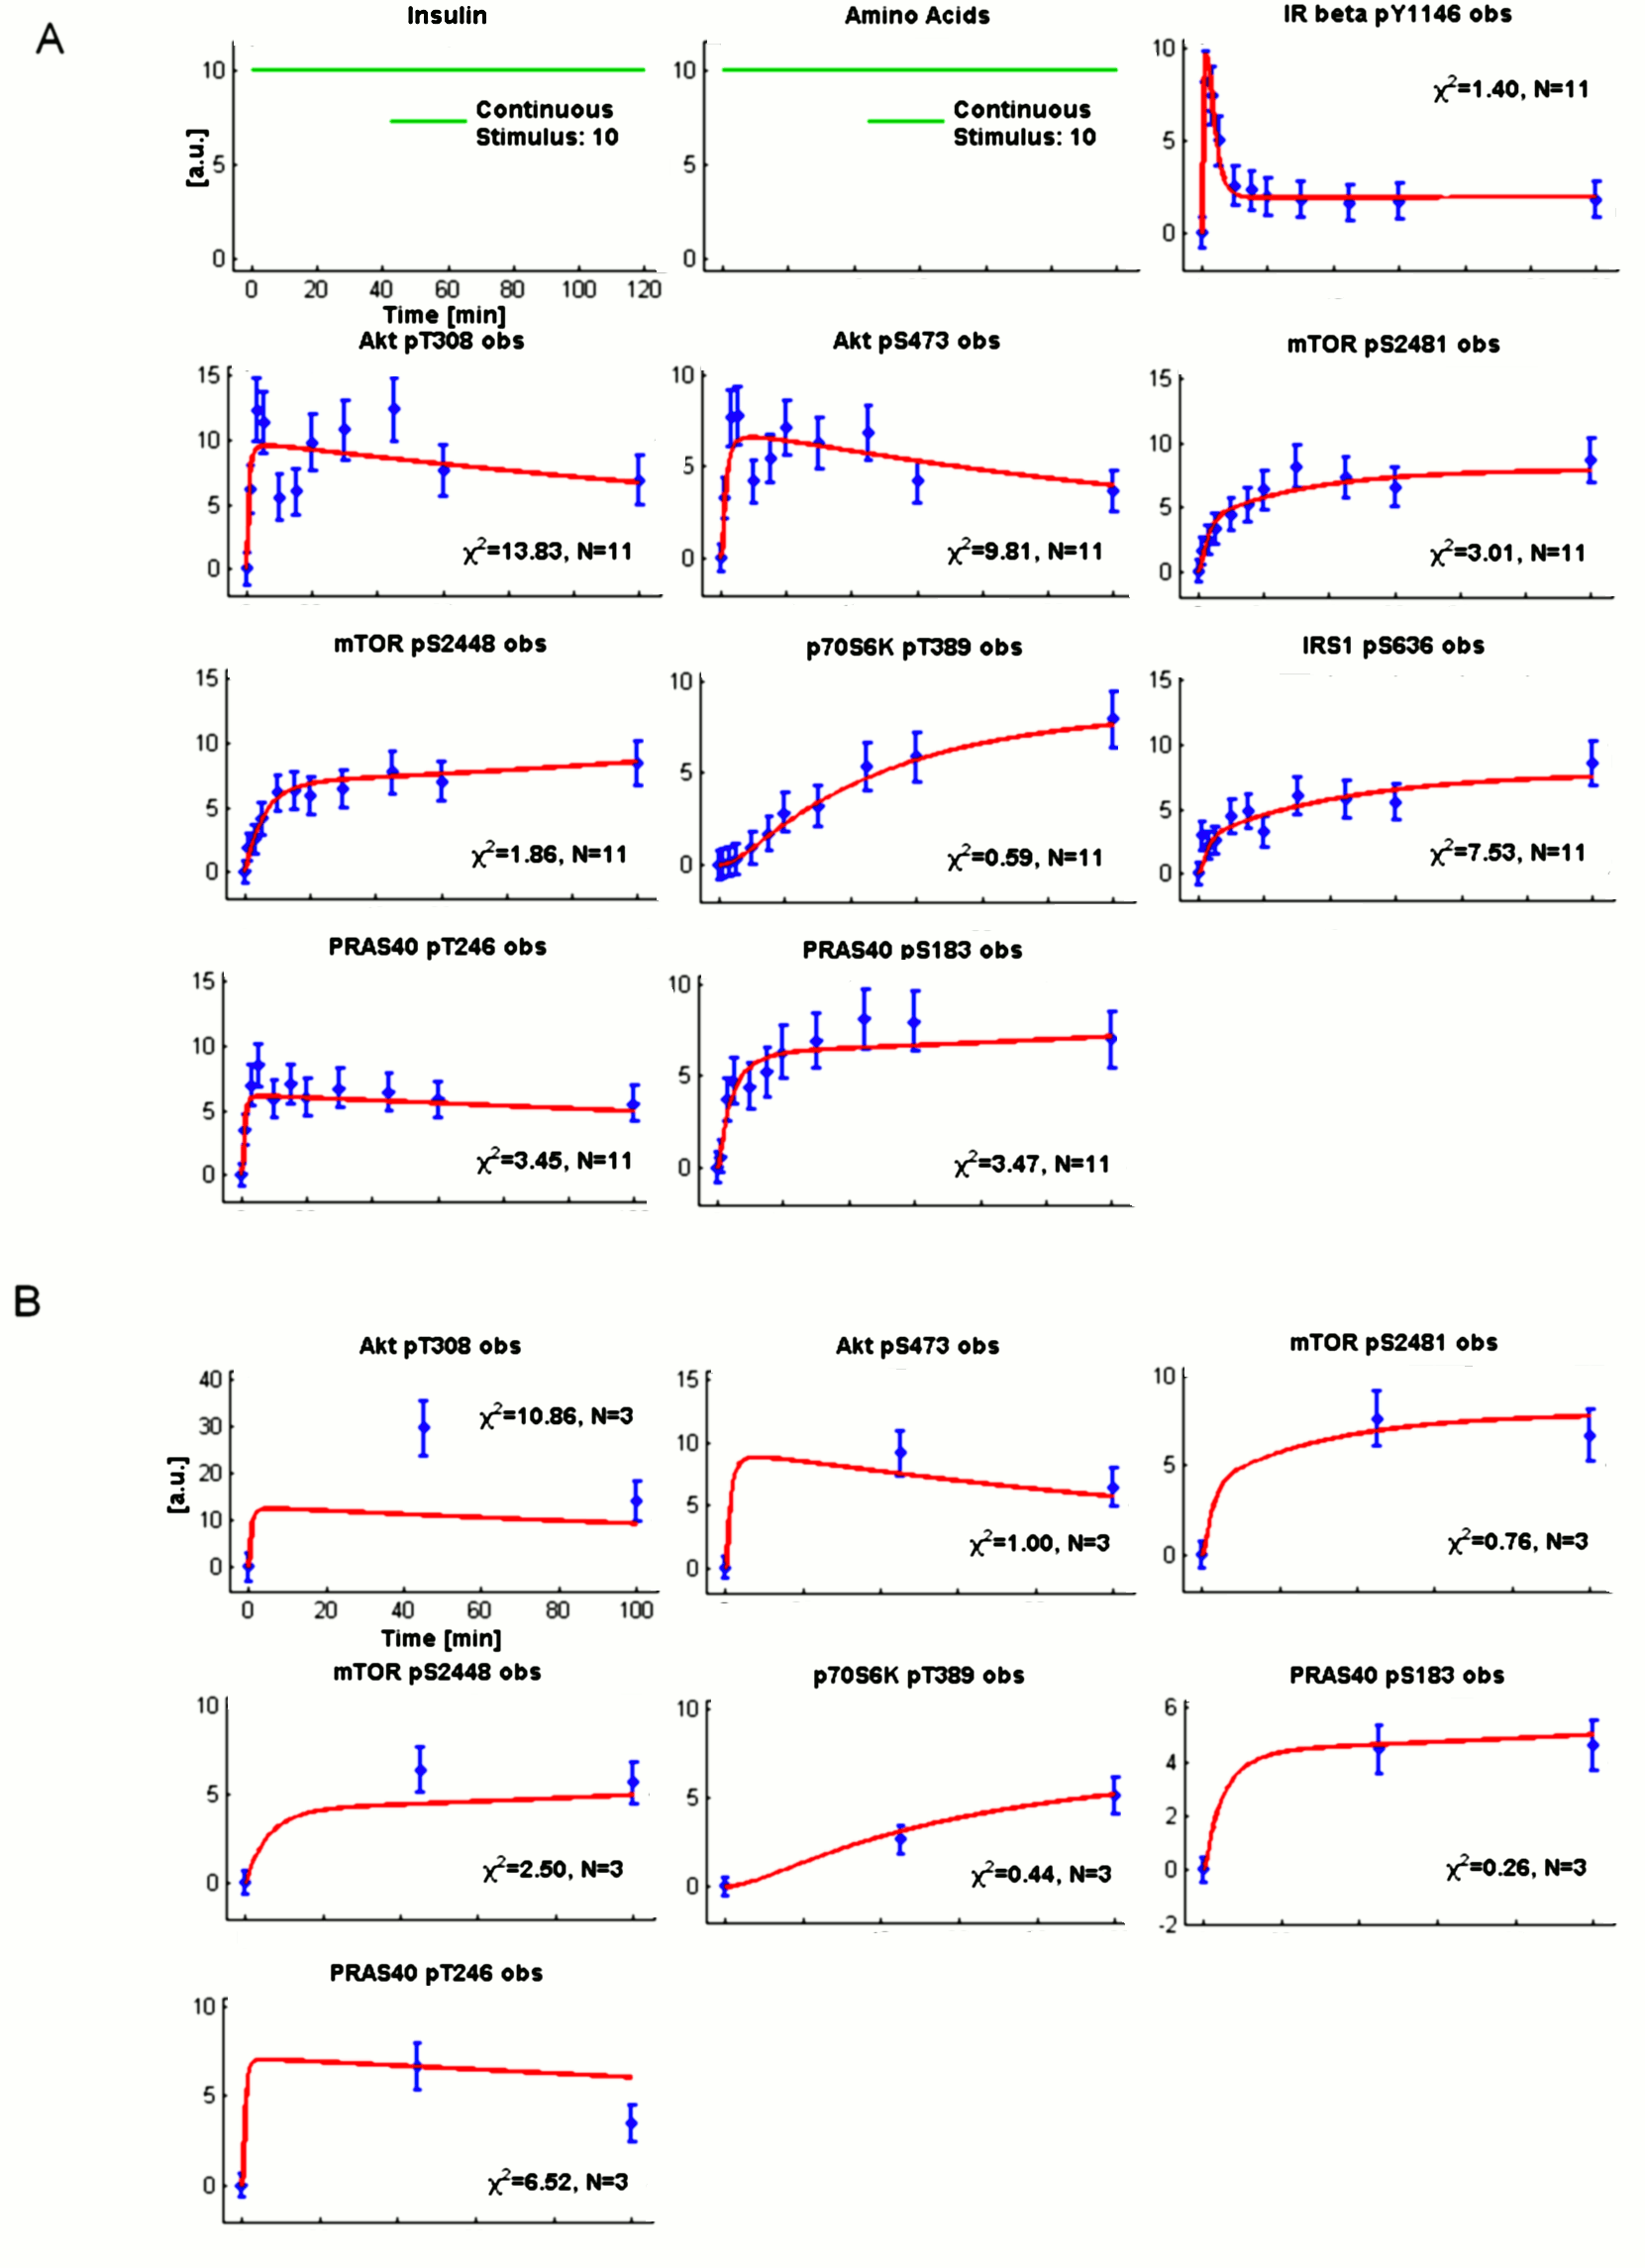
\includegraphics[width=4.60in]{fj_sb_12_0009_supp_fig_3.png}
		%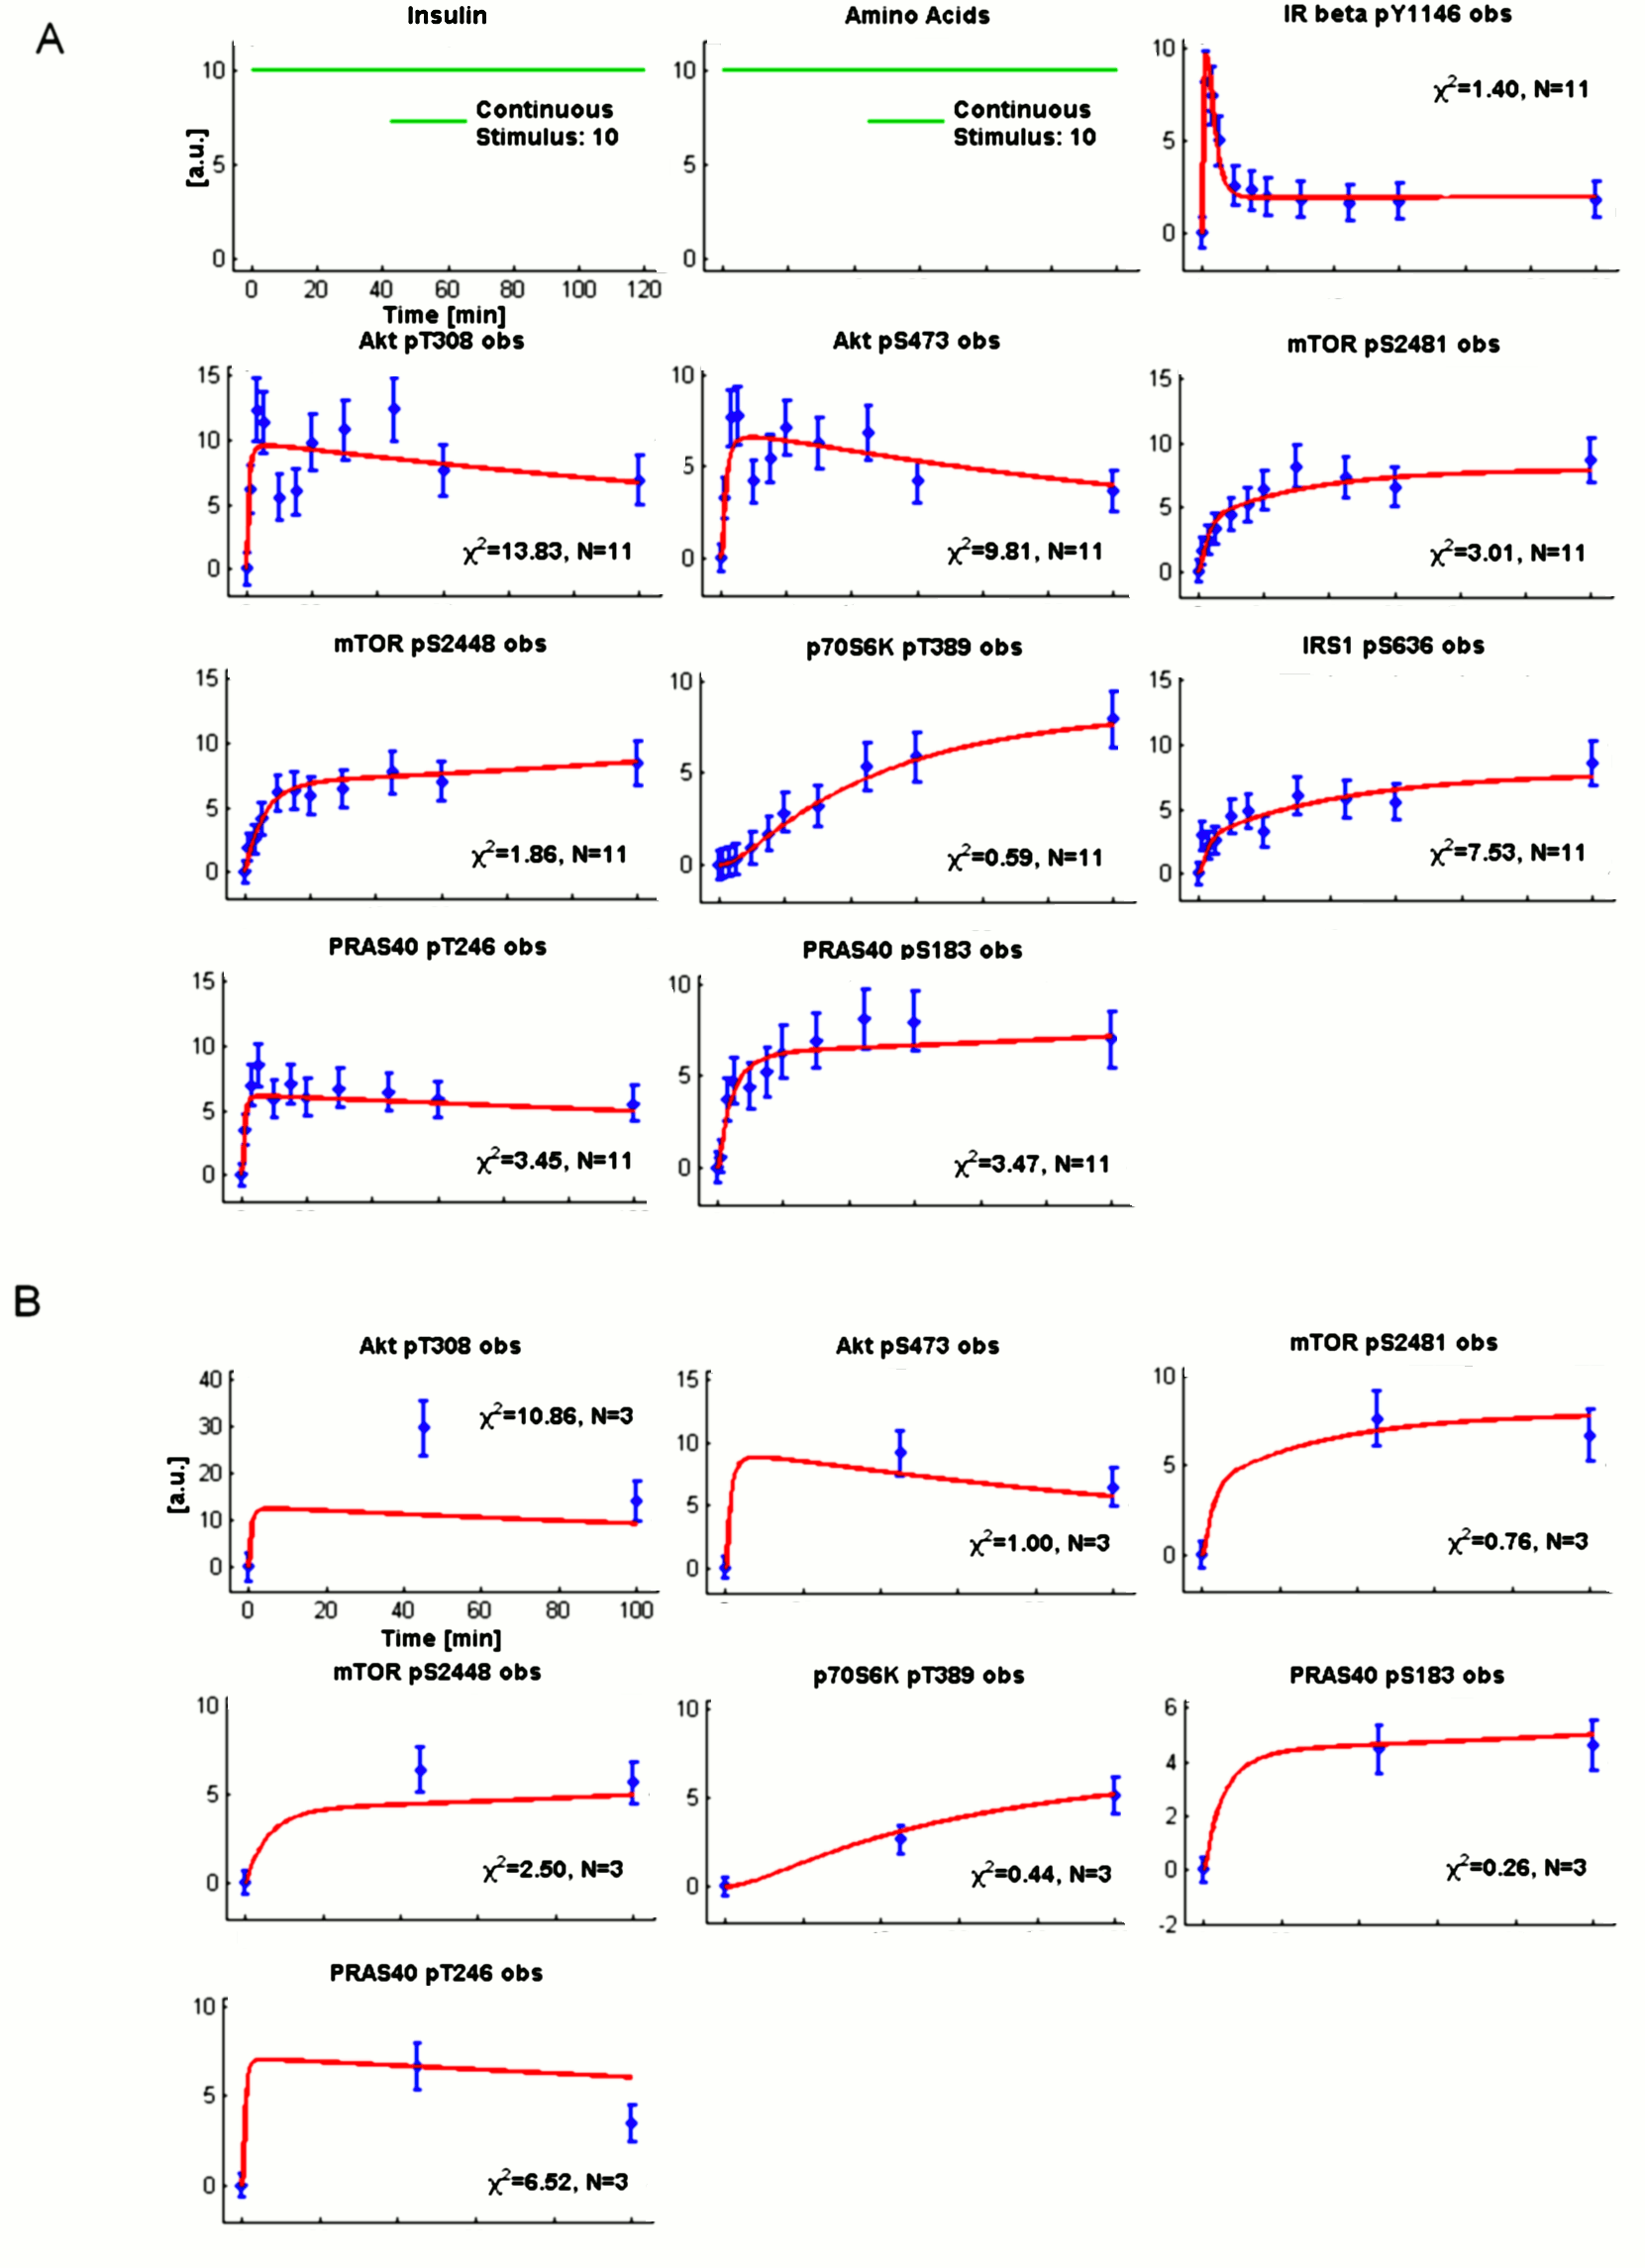
\includegraphics[scale=0.9]{fj_sb_12_0009_supp_fig_3.png}
		\caption[Additional simulated versus experimental time courses for IRS1-induced AMPK model (Hypothesis 3)]{Additional simulated versus experimental additional time courses for IRS1-induced AMPK model (Hypothesis 3). (A) Main data set used for parameter estimation. Simulated (red lines) versus experimental data (blue points) are plotted for nine wild type (WT) readouts along the insulin-TOR network upon amino acids/insulin induction. (B) Additional data set used for parameter estimation. Experimental data for seven readouts for a Raptor knock down (KD) upon amino acids/insulin induction. Experimental data error bars indicate standard error of the mean (SEM) calculated from four repetitions. Goodness-of-fit $\chi^2$ is reported for each plot along with the number of measured time points. \emph{In vitro} experiments were performed by Annika Sonntag, Freiburg University, Germany.}
		\label{fig:fj_sb_12_0009_supp_fig_3}
	\end{center}
\end{figure}
\clearpage

\begin{figure}[tb]
	\begin{center}
		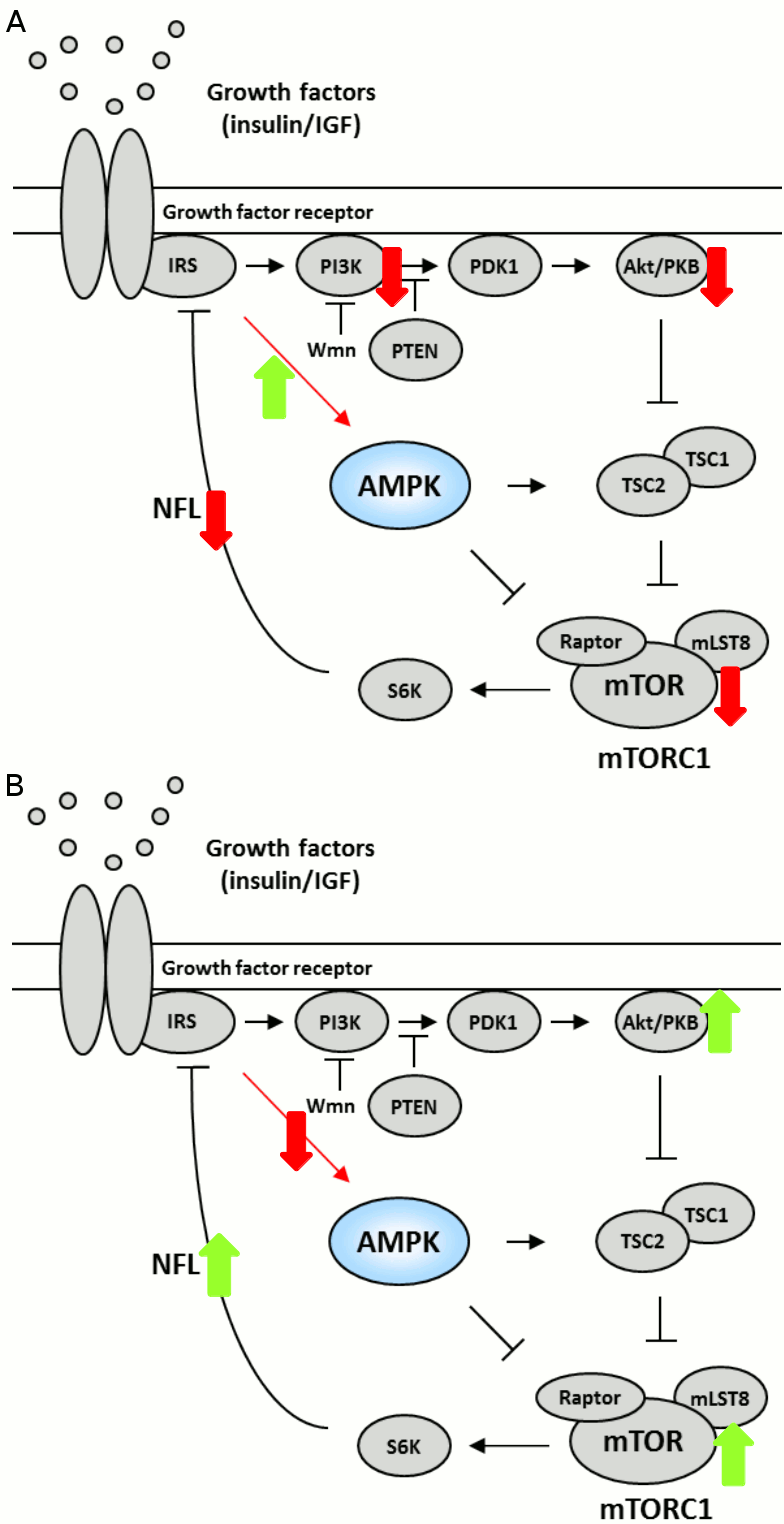
\includegraphics[width=3.4in]{schematic_diagrams_tests.png}
		%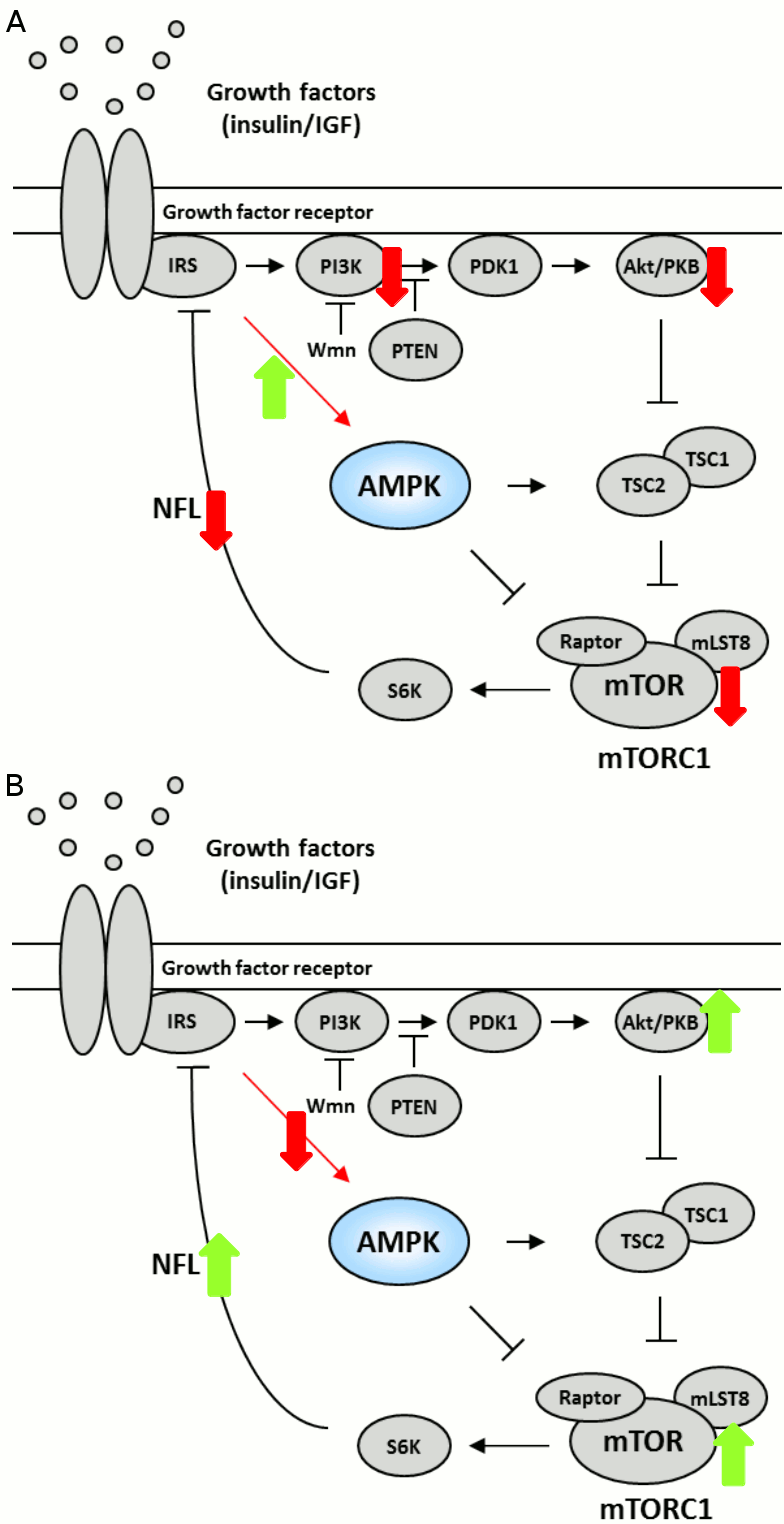
\includegraphics[scale=1.4]{schematic_diagrams_tests.png}
		\caption[Schematic diagrams for testing hypotheses ranking]{Schematic diagrams for testing hypotheses ranking. (A) IRS overexpression induced AMPK and TSC1/TSC2 activity directly and indirectly by inhibiting the negative feedback loop (NFL). In addition, AMPK was also positively regulated by either inhibiting PI3K with Wortmannin or overexpressing PTEN. (B) Constitutively active Akt inhibited AMPK by hyperactivating the NFL. Wmn: Wortmannin. Figures adapted from \citep[Fig. 5A]{Sonntag2012}.}
		\label{fig:paper2_schematic_diagrams_tests}
	\end{center}
\end{figure}
\clearpage



\begin{figure}[tb]
	\begin{center}
		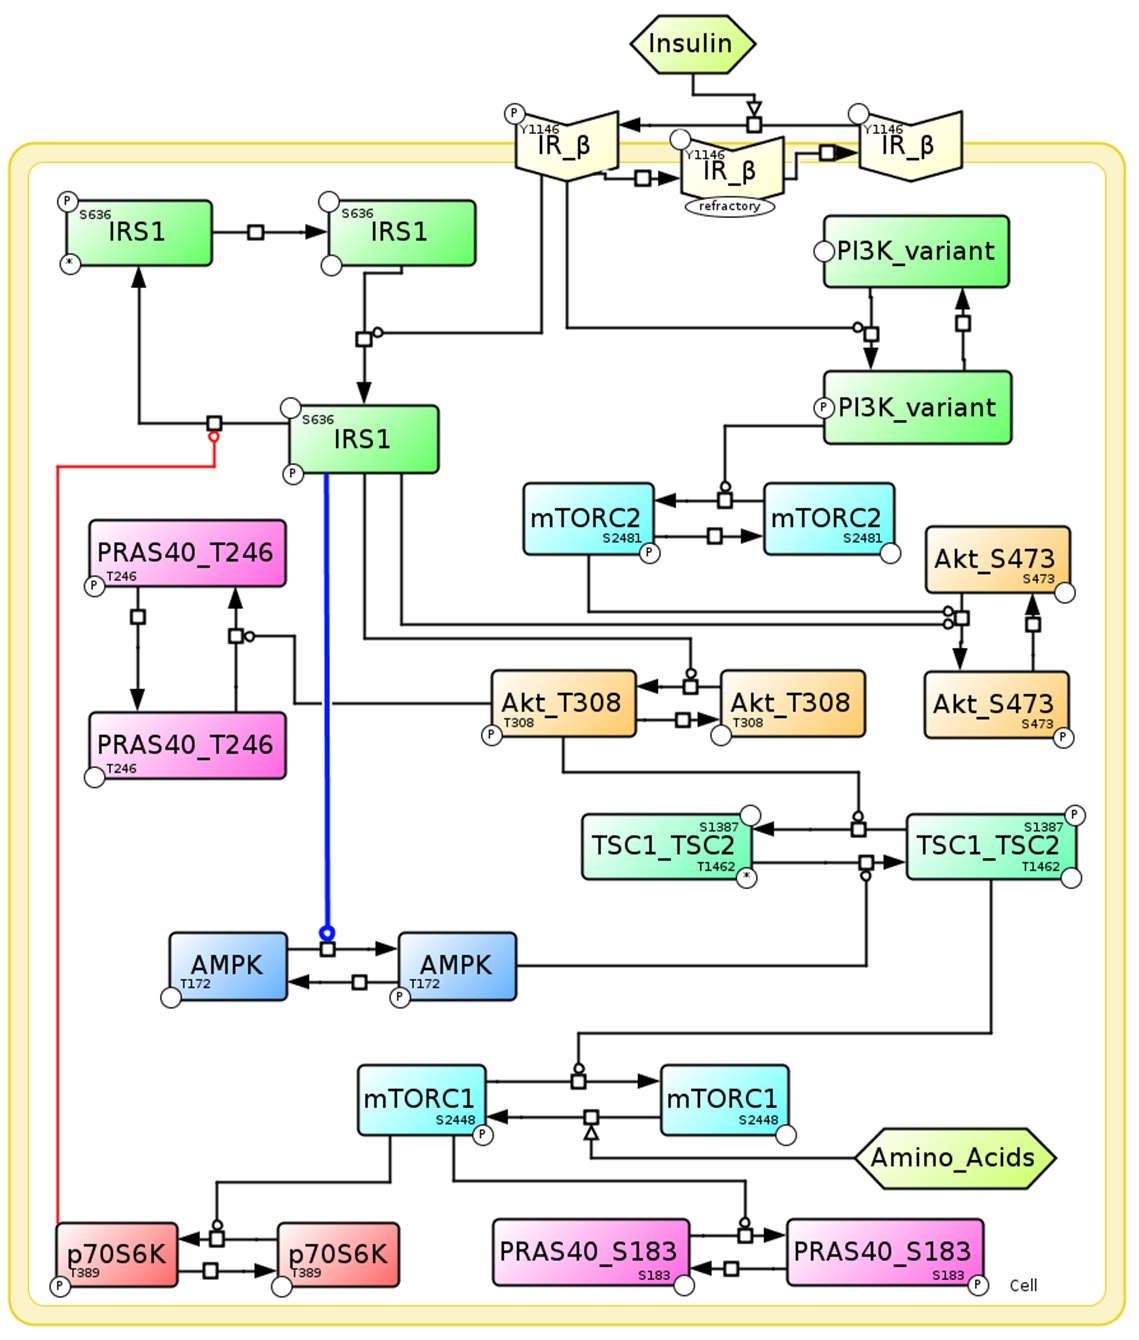
\includegraphics[scale=1.2]{fj_sb_12_0009_fig_5.jpg}
		\caption[IRS is required for AMPK induction by insulin (Hypothesis 3)]{IRS is required for AMPK induction by insulin (Hypothesis 3). Graphical model of the insulin induced mTORC1 pathway in SBGN notation, including IRS dependent AMPK induction. Importantly, the negative feedback loop (NFL) via IRS targets not only PI3K but also AMPK.}
		\label{fig:fj_sb_12_0009_fig_5}
	\end{center}
\end{figure}
\clearpage






%\section{Tables}
%\label{paper2-sec:Tables}

\begin{table}[tb]
	\begin{center}
		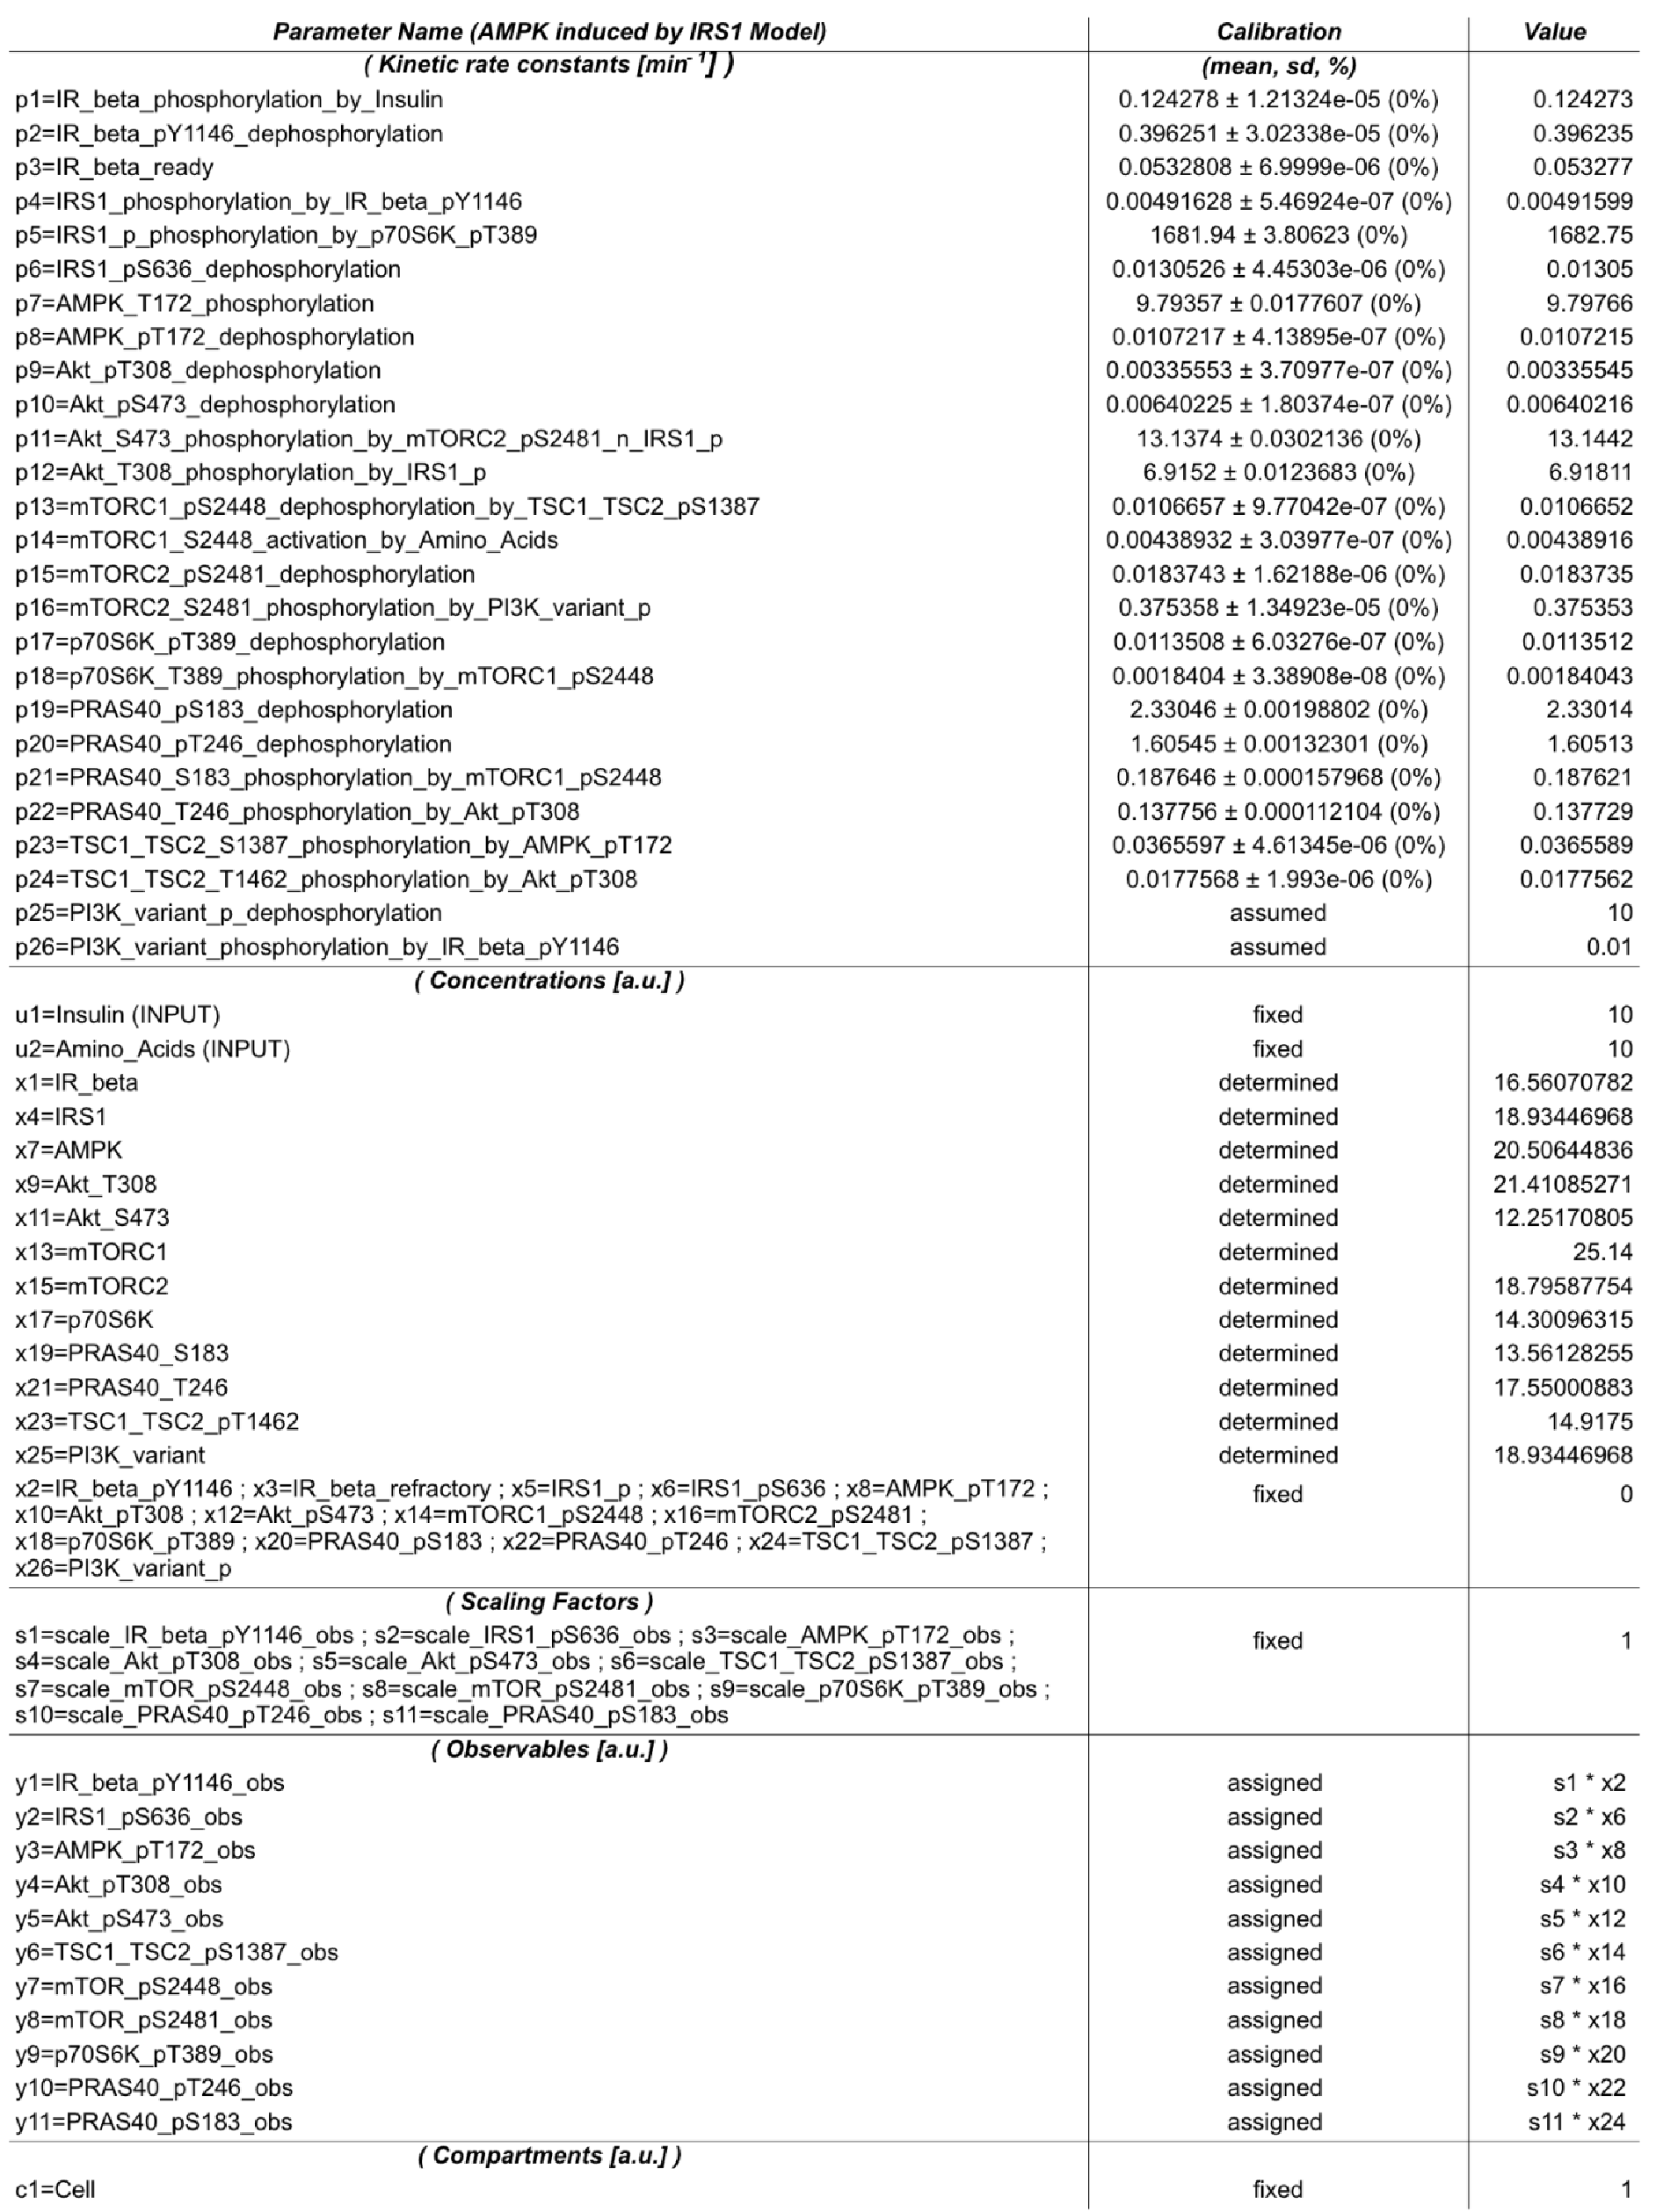
\includegraphics[scale=0.26]{fj_sb_12_0009_fig_t1.png}
		\caption[Parameter table for the IRS1-induced AMPK model (Hypothesis 3)]{Parameter table for the IRS1-induced AMPK model (Hypothesis 3). The estimated kinetic rate constants together with the species concentrations are provided. The mean, standard deviations and percent of standard deviation over the mean, computed over the 50\% of the best fits, are also indicated. These statistics shows that all the 24 estimated parameter could be fixed at the first round of calibration. Scaling factor parameters and observable variables are also indicated.}
		\label{tab:fj_sb_12_0009_fig_t1}
	\end{center}
\end{table}
\clearpage

\begin{table}[tb]
	\begin{center}
		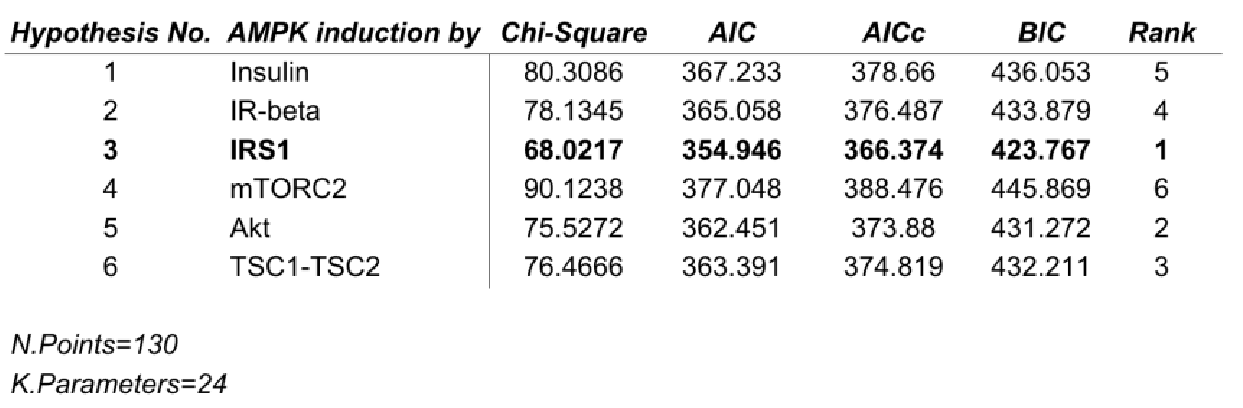
\includegraphics[scale=0.3]{fj_sb_12_0009_fig_t2.png}
		\caption[Statistical ranking of the models]{Statistical ranking of the models. Quality of fitting measures were used to determine a ranking of the investigated models. IRS1-induced AMPK model (Hypothesis 3) showed the lowest $\chi^2$ value, indicating that this model was the most probable. AIC, AICc and BIC values are reported as additional measures.}
		\label{tab:fj_sb_12_0009_fig_t2}
	\end{center}
\end{table}
\clearpage




% ------------------------------------------------------------------------


%%% Local Variables: 
%%% mode: latex
%%% TeX-master: "../thesis"
%%% End: 
